%
%	final_report.tex
%
%	Final Report Outline
%
%	John Hughes and Michael Jean
%	University of Manitoba
%

\documentclass[english]{scrreprt}

\KOMAoptions{fontsize=11pt}
\KOMAoptions{paper=letter}

%%% Preamble

%
%	preamble.tex
%
%	Final Report: Document Preamble
%
%	John Hughes and Michael Jean
%	University of Manitoba
%

\usepackage[T1]{fontenc}
\usepackage[utf8x]{inputenc}

\setcounter{secnumdepth}{3}
\setcounter{tocdepth}{3}

\usepackage{amsmath}
\usepackage{array}
\usepackage{babel}
\usepackage{float}
\usepackage[letterpaper]{geometry}
\usepackage{graphicx}
\usepackage{graphics}
\usepackage{lastpage}
\usepackage{tikz}
\usepackage{tikz-timing}[2009/05/15]
\usepackage{subfigure}
\usepackage{tabularx}
\usepackage{array}
\usepackage{flafter,fnpos}
\usepackage{booktabs}
\usepackage{supertabular}
\usepackage{setspace}

\usepackage[binary]{SIunits}

%\usepackage[square,authoryear,sort&compress]{natbib}
\usepackage[numbers, square, comma, sort&compress]{natbib}

\usepackage{nomencl}
\makenomenclature

\usepackage{fancyhdr}

%%% Set Margins
\setlength{\hoffset}{0.5in}
\oddsidemargin=0pt
\setlength{\topmargin}{0pt}
\setlength{\marginparwidth}{0pt}
\setlength{\marginparsep}{0pt}
\setlength{\textwidth}{6in}
\setlength{\textheight}{600pt}
\setlength{\footskip}{20pt}
\setlength{\headsep}{15pt}

\setlength{\parskip}{\medskipamount}
\makeatletter

% Tikz styles

% Define the arm and angle options
\def\myarm{1cm}
\def\myangle{0}
\tikzset{
  arm/.default=1cm,
  arm/.code={\def\myarm{#1}}, % store value in \myarm
  angle/.default=0,
  angle/.code={\def\myangle{#1}} % store value in \myangle
}

% Define the myncbar to path
\tikzset{
    myncbar/.style = {to path={
        % We need to calculate a couple of coordinates to help us draw
        % the path. 
        let
            % Same as (\tikztotarget)++(\myangle:\myarm)
            \p1=($(\tikztotarget)+(\myangle:\myarm)$)
        in
            -- ++(\myangle:\myarm) coordinate (tmp)
            % Find the projection of the (tmp) coordinate
            % on the line from the target to p1
            -- ($(\tikztotarget)!(tmp)!(\p1)$)
            -- (\tikztotarget)\tikztonodes
    }}
}

\tikzstyle{red shiny} = [draw=red!50!black!50, top color=white,bottom color=red!50!black!20, drop shadow]
\tikzstyle{blue shiny} = [draw=blue!50!black!50, top color=white,bottom color=blue!50!black!20, drop shadow]
\tikzstyle{grey shiny} = [draw=gray!50!black!50, top color=white,bottom color=gray!50!black!20, drop shadow]

\tikzstyle{start} = [grey shiny, signal, signal to=east, draw]
\tikzstyle{end} = [grey shiny, signal, signal from=east, draw]
\tikzstyle{decision} = [ blue shiny, diamond, text width=1cm, text badly centered, inner sep=0pt]

\tikzstyle{module} = [ blue shiny, rectangle, very thick]

\tikzstyle{block} = [ red shiny, rectangle,
		      %minimum height=3em,
		      %minimum width=6em,
		      %inner sep=0.5em,
		      text width=2cm,
		      text centered]
\tikzstyle{bus} = [coordinate]
\tikzstyle{input} = [coordinate]
\tikzstyle{output} = [coordinate]

\tikzstyle{small block} = [ red shiny,
		      rectangle,
		      very thick,
		      %minimum height=3em,
		      %minimum width=3em,
		      inner sep=0.5em,
		      text width=1cm,
		      text centered]

\usepackage[
  unicode=true,
  pdfusetitle,
  bookmarks=true,
  bookmarksnumbered=true,
  bookmarksopen=false,
  breaklinks=false,
  pdfborder={0 0 0},
  backref=false,
  colorlinks=false
] {hyperref}

\renewcommand{\baselinestretch}{1.0}

\begin{document}
\pagenumbering{roman}

%%% Title Page

\subject{Design and implementation of a distributed automotive sensor/actuator network}
\title{Final Report}

\author{John Hughes\\ Michael Jean\\ Group Advisor: Dr. W. Kinsner}

\maketitle

%\newpage
%\phantomsection \label{visual_abstract}
%\addcontentsline{toc}{chapter}{Visual Abstract}
%Visual Abstract

\begin{abstract}
\begin{abstract}
  Statement of the problem
• Procedures and methods used
• Results
• Conclusions

The problem is tackled with a distributed divide and conquer approach: and architecture of four seperate electronic modules is devised. Each module is designed to communicate with the others as well as pre-existing modules.

Four prototype modules were constructed with custom-designed printed circuit boards.

Final testing of the engine and transmission module, and the braking module was not conducted since the completed SAE vehicle intended for installation was not yet available.
\end{abstract}


\end{abstract}

\chapter*{Contributions}
\addcontentsline{toc}{chapter}{Contributions}
Contributions

\chapter*{Acknowledgements}
\addcontentsline{toc}{chapter}{Acknowledgements}
Acknowledgements

\renewcommand{\contentsname}{Table of Contents}
\tableofcontents{}

\newpage
\phantomsection \label{listoffig}
\addcontentsline{toc}{chapter}{List of Figures}
\listoffigures

\newpage
\phantomsection \label{listoftab}
\addcontentsline{toc}{chapter}{List of Tables}
\listoftables

\newpage
\phantomsection \label{nomenclature}
\addcontentsline{toc}{chapter}{Nomenclature}
\printnomenclature{}

\newpage

\pagenumbering{arabic}
%\setstretch{1.5}

\chapter{Introduction\label{cha:introduction}}

\section{Formula SAE}

Formula SAE\nomenclature{SAE}{Society of Automotive Engineers} is an engineering student design competition organized by the Society of Automotive Engineers dating back to 1978 \cite{fsaehistory}. Students from the University of Manitoba have participated in the competition almost every year since 1985. The competition consists of designing and constructing a small, open-wheeled, formula-style race car.

The Formula SAE vehicle is a performance car built with the primary goal of doing well in the dynamic events at the yearly competitions. These events test the vehicles' abilities in acceleration, braking, and handling. 

\section{Motivation}

Many of the issues that directly affect the teams' performance at competition relate to driver training, feedback, and the tuneability of the car. Most of the mechanical systems on the car must currently be imprecisely hand-tuned, and are packaged in hard to reach places, and require body panels or the seat to be removed for access.

Our overall goal is thus to improve the precision, adjustability, and repeatability of adjustment, of various important mechanical systems in the car, and to improve the efficiency of testing. Highly desirable is a shorter driver-feedback-tuning loop in order to eliminate overshoot and undershoot in tuning, and to avoid other external disturbances.

A second major goal is to improve upon the transmission control systems of previous years' designs.

\section{Problem Definition}

The goal of this work is to tackle several distinct issues on the 2010 Formula SAE Vehicle:

\begin{itemize}
 \item electronic control of the transmission is to be quantifiably improved over previous years' control;
 \item engine output power will be increased under specific conditions by dynamically varying the intake geometery;
 \item the front-to-back brake bias will be electronically adjustable;
 \item data from on-board systems will be accessible wirelessly;
 \item an easy to use yet powerful user interface will allow the driver to control on-board systems and provide feedback of critical vehicle parameters.
\end{itemize}

Improving electronic control of the transmission should result in decreased gear shift times, improved mechanical reliability of the transmission, decreased driver effort, and the elimination of any manual mechanical interaction with the transmission by the driver.

Successful introduction of variable intake geometery will widen the peak torque output from the engine, improving acceleration.

Electronically adjustable brake bias will improve tuneability by allowing the brake bias to be adjusted on the fly, even while the vehicle is in motion. It should reduce the need for manual adjustment and calibration.

Wireless telemetry data will improve vehicle performance and reliability by relaying critical vehicle operation data from various sensors to the pit crew, who can then make decisions regarding the various vechile parameters. The module should be able to broadcast to the pit area while the vehicle is competing in all of the dynamic events. It must operate with a minimum of data loss despite the distance and motion of the vehicle relative to the pit crew.

The driver interface should reduce driver effort and improve vehicle performance by allowing the driver to manage all the tuneable vehicle parameters from a simple interface located on the steering wheel, and by providing the driver with real-time feedback from the various vehicle sensors in an easy-to-read format.

\section{Strategy}

To meet the requirements of the project, a networked 4-module architecture was chosen. The architecture will be described in further detail in Chapter \ref{ch:design}, however to aide the reader in understanding the scope of the project, the modules will be introduced here. These 4 modules are:

\begin{itemize}
\item the transmission and engine control module;
\item the brake bias adjustment module;
\item the wireless telemetry module; and
\item the driver interface module.
\end{itemize}

The components selected should not aversely affect the weight of the vehicle or dramatically increase the complexity of the mechanical systems, rather they should only require minimal mechanical adaptations to achieve the tuneability and performance goals outlined. As the team receives funding exclusively through 3rd-party sponsorship, the components selected should not dramatically increase the overall cost of the vehicle.

Additionally, to facilitate testing of the network, a CAN testing module will be developed, consisting of an off-the-shelf AT90CAN128 development board, and custom software.

The design and implementation of each module required several steps. 

Absolute requirements and specifications for system parameters were first estabilshed. The electromechanical interface linking the control systems and mechanical systems were decided between our group and the mechanical engineers responsible for each respective system. The measurement requirements from the mechanical systems were be established and the appropriate sensors chosen.

Appropriate components for the electronic modules were chosen, and circuits designed. The schematic of each module was designed and an appropriate printed circuit board layed out. The boards were manufactured and populated with components. Each board must be tested to ensure all wiring is correct and the functionality of all the components is correct.

Firmware for each module must be implemented once the hardware design is finished. Software libraries for various components must be written and tested. The libraries must be combined with a high-level control algorithm for each module.
 
Each module must be tested in isolation to ensure proper functionality. The modules must then be interconnected and tested again.

\section{Outline of Thesis}

This thesis is organized into 8 chapters. After this introductory chapter, Ch. \ref{cha:background} provides background information describing the vehicle systems we will interact with, the problems associated with these systems we are attempting to solve, and a description of previous efforts to solve these problems. In Ch. \ref{cha:goals_and_requirements} the goals and requirements of the design work will be specified for each of the areas described in Ch. \ref{cha:background}. Chapter \ref{cha:design} describes our design to meet these requirements. Chapter \ref{cha:implementation} describes our implementation of the design.

\chapter{Background}


\section{Transmission}


\subsection{Overview}

Brief {}``what is transmission''

Shifting speed and dexterity required

Stall avoidance

-one chance to restart during race

-sensitivity to stalling

launching the car, etc.


\subsection{Mechanical Systems}

Simple descriptions


\subsubsection{Clutch}


\subsubsection{Gear Selection}


\subsection{Previous Implementations and Shortcomings}

How, challenges, etc.


\subsubsection{Electropneumatic Actuation}


\subsubsection{Gear Position Sensing}


\subsubsection{Neutral Sensing}


\section{Engine}


\subsection{Overview}

brief {}``what is engine'', honda cbr, etc.

maximise power output (performance application)

torque power curve, etc.


\subsection{Intake and Exhaust}

Intake background, pressure waves, etc. Torque curve depends on length, 


\subsection{Research and Modelling of Variable Length Intake}

present research done by others on team, quantified runner length
dependence

intake length changes power

quantified length versus power on actual vehicle

chose optimal intake length

proposed variable length intake system for future work


\subsection{Starting System}

current requirements, starter motor, etc.


\section{Braking}


\subsection{Overview}

Idea of braking and force distribution


\subsection{Mechanical Systems}


\subsubsection{Independant Hydraulic Systems}


\subsubsection{Balance Bar}


\subsection{Adjustment Difficulties}

Competition problems, manual adjustment difficulty, scope of adjustment,
tuneability lag


\section{Telemetry}


\subsection{Overview}

Why is telemetry necessary? Sensors, data, etc.


\subsection{ECU}

A specialized third-party component called the \emph{Engine Control Unit} (ECU) controls the fuel injector and spark coil systems that in turn control the combustion cycle of the engine. The particular model of ECU used by the Formula SAE car is the S80Pro from DTAFast \cite{s80pro}. The ECU uses the O$_{2}$, MAP, cam position, and crank position sensors to adjust the fuel injector and spark coil timings. This keeps the engine running smoothly. The ECU features a traction control system that monitors wheel slip and cuts spark and fuel to provide traction when one of the wheels is slipping. The ECU also collects the various sensor readings and makes them available to other electronic devices at a fixed frequency through a shared data bus. 

\begin{figure}[H]
\centering
%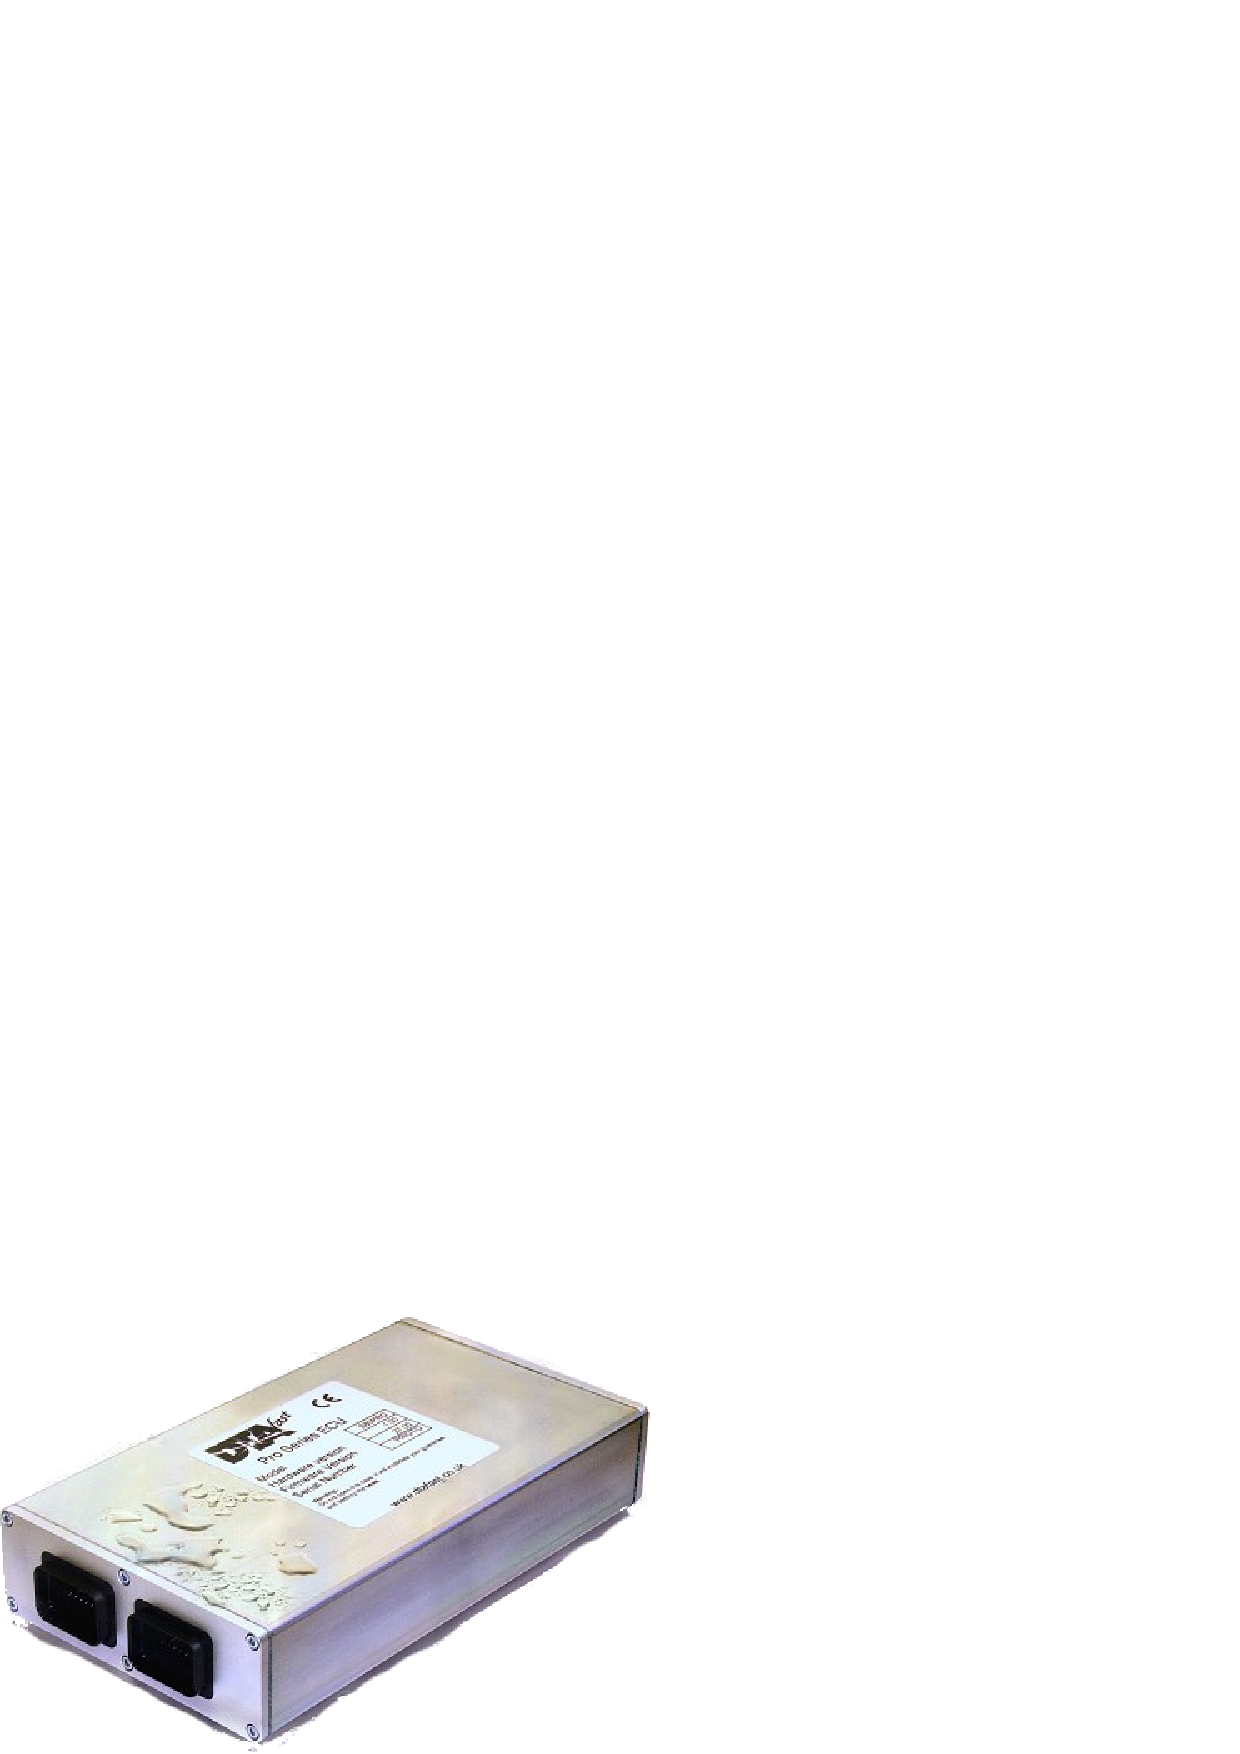
\includegraphics[scale=0.5]{Figures/s80.png}
\caption{The DTAFast S80Pro engine control unit.}
\label{fig:s80pro_product}
\end{figure}

\subsubsection{ECU Data interface}
\label{sec:ecu_data} 

The ECU provides 2 digital communication methods:
\begin{itemize}
 \item An RS-232 link is used by the software that DTA provides for tuning and controlling the ECU. The serial protocol that the software uses is proprietary and undocumented.
 \item A read-only CAN bus interface that emits ECU data at a fixed frequency. The message format for the CAN data is documented in Appendix \ref{cha:ecu_can_spec}.
\end{itemize}
 
\nomenclature{RS-232}{Recommended Standard 232, a byte-oriented serial communications protocol, typically asynchronous.}


\subsection{DAC}

Another specialized third-party component called the \emph{Data Acquisition Device} (DAC) is used to log and relay sensor data to other electronic devices.

The particular DAC used is the model DL1 from Race Technology \cite{DL1Dsheet}. The DL1 is an expandable data logger with built-in 20-Hz GPS and 3-axis accelerometer.

\subsubsection{DAC Data Interface}

Race Technology provides a software suite that communicates with the DAC using a documented serial protocol. Every item that the DAC logs is output to its own channel in real time on the serial port. It is also possible to configure the software to recognize new channels for arbitrary types of data.

\begin{figure}[H]
\centering
%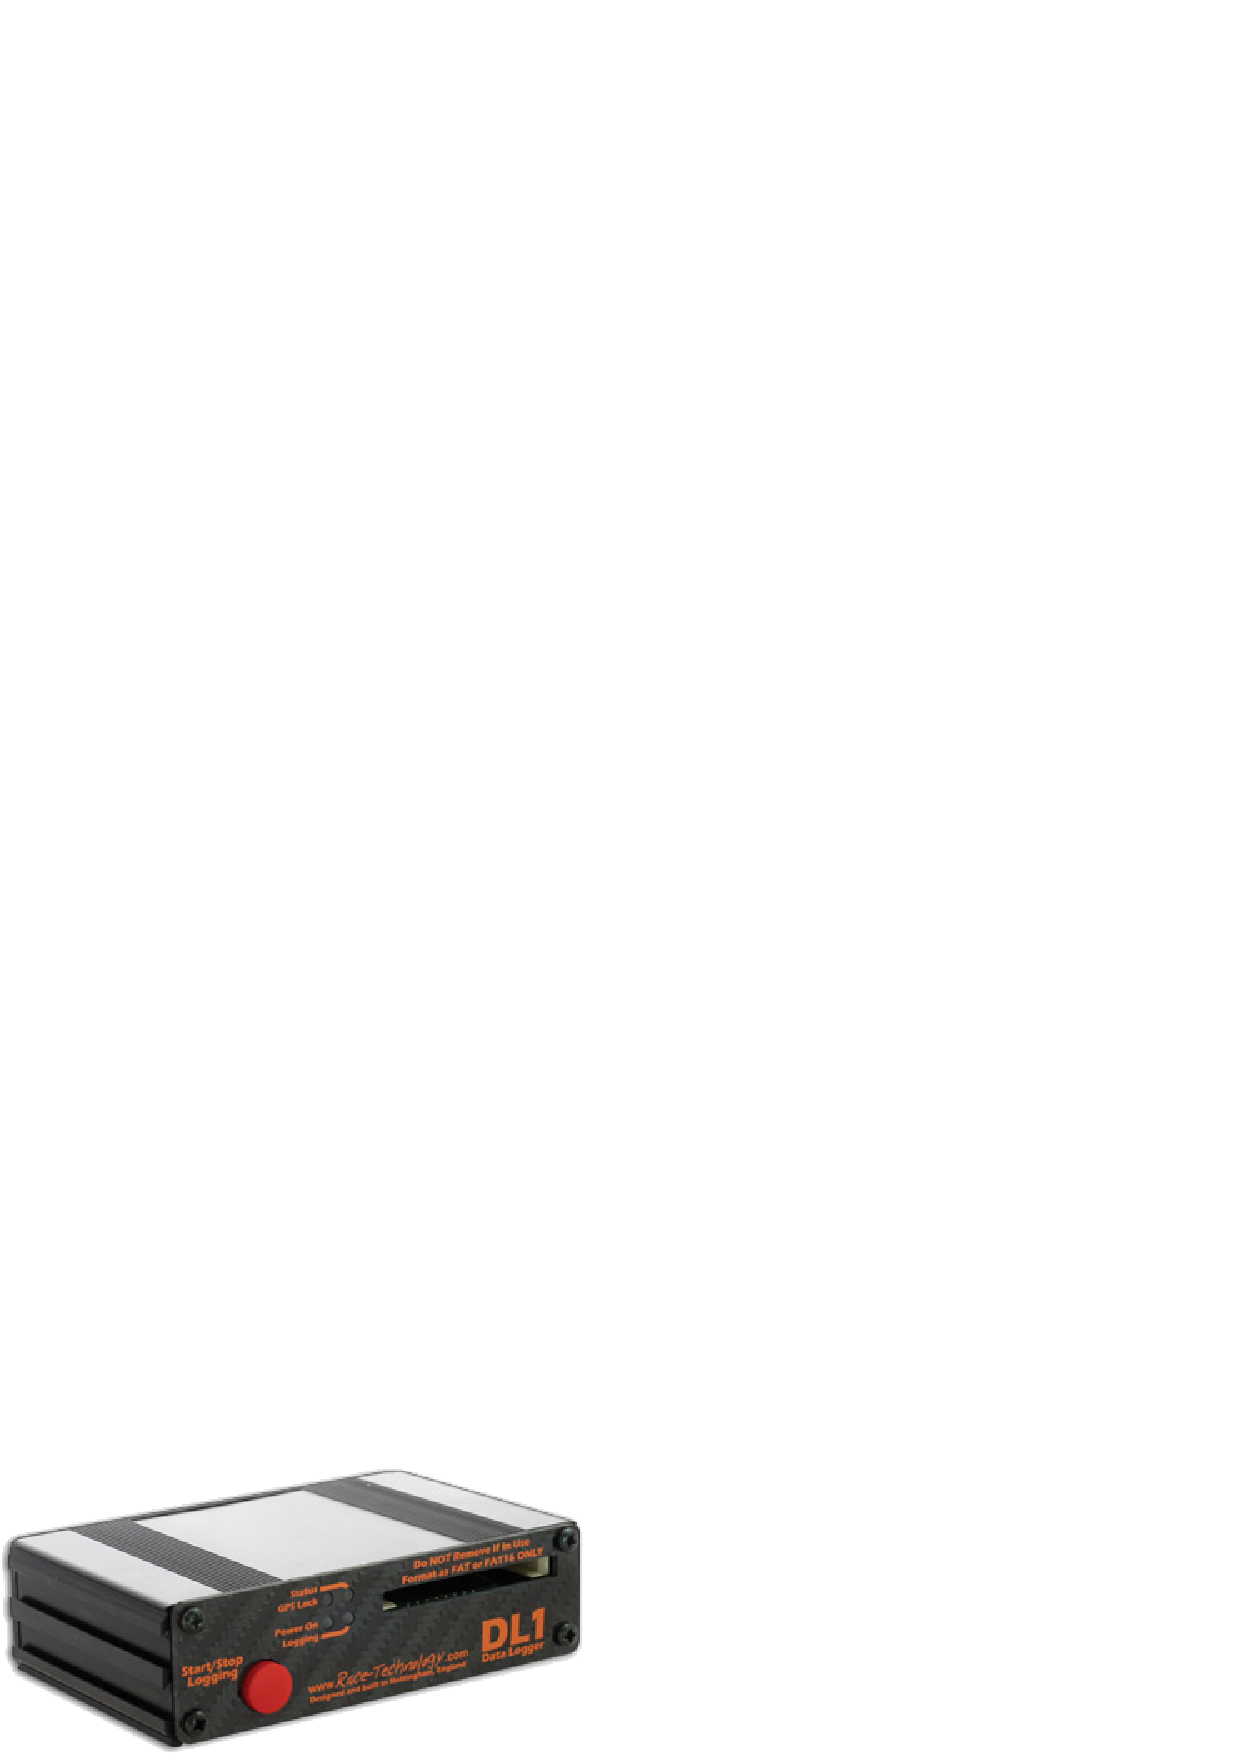
\includegraphics[scale=0.5]{Figures/dl1.png}
\caption{The Race Systems DL1 data acquisition device.}
\label{fig:dl1_product}
\end{figure}


\subsection{Previous Implementations and Shortcomings}


\subsubsection{Cellular Link}


\subsubsection{Off-the-Shelf XBee Link}

Both of these only worked with one device, weren't reliable, etc.


\section{Driver Interface}


\subsection{Overview}

Driver and crew needs easy access to data, easy control of on-board
systems


\subsection{Driver Controls}


\subsubsection{Transmission Control}

Upshift/Downshift

Activate other trans. control features, neutral find, etc., launch


\subsubsection{Engine Control}


\subsection{Vehicle Diagnostics}


\subsubsection{Critical Indicators}

Overheating, oil pressure, etc.


\subsubsection{Supplimentary Indicators}

information about telemetry, shift control, etc.


\subsection{Previous Implementations and Shortcomings}

\chapter{Goals and Requirements\label{cha:goals}}

The guiding principle for the project is to incorporate changes that will improve the team's standing at competition. This can be achieved by improving the vehicle's performance, and by reducing the demand on the driver so that they may focus more on driving the vehicle. This chapter outlines the goals and requirements to which our design is built and measured against.

Each of the five major systems introduced in Ch. \ref{cha:background} have a set of goals and requirements associated with them. The limitations and shortcomings of each system that were encountered in previous years will be addressed. When possible, quantitative targets will be set based on research and recommendations from the mechanical engineers involved with the vehicle.

 \section{Engine}

The main goal of the engine system is to optimize the peak torque output of engine. This can be accomplished with a variable-length intake system, as suggested by Groening in \cite{LucasIntake}. Achieving this requires the ability to monitor the current engine speed and to mechanically adjust the runner lengths as needed.

\begin{itemize}
\item Automatically adjust the variable-length two-position intake to optimize peak torque output.
\item The intake runner length should be chosen automatically by determining the best position to optimize output power.
\item Changing the intake runner length positions should take no more than \unit{150}{\milli\second}.
\end{itemize}

\section{Transmission and Drivetrain}

The overall goal for the transmission and drivetrain systems is to improve shift time and accuracy while reducing the effort required by the driver. To achieve this goal requires modifying and improving the existing electro-pneumatic system by improving both the pneumatics and the electronic transmission control system. 

\subsection{Shifting}

\begin{itemize}
\item Reduce the time to change gears to less than \unit{100}{\milli\second}. 
\item Implement a neutral-finding feature that will automatically downshift from the current gear to neutral in the shortest amount of time.
\item Implement an automatic up-shift feature that will up-shift the transmission without driver intervention to obtain the best possible acceleration.
\item Provide the ability to enable or disable the neutral-finding and automatic up-shifting features from the cockpit.
\end{itemize}

The average force required to actuate the shift lever on the CBR600f4i was measured using a fish scale to be \unit{5.42}{\newton\metre}. Any actuation method designed will need to be able to produce this torque, plus a factor of safety to account for wear and inconsistency.

\begin{itemize}
\item The shift lever actuator must be able to apply a minimum of \unit{6.00}{\newton\metre} of torque.
\end{itemize}

\subsection{Clutch Control}

\begin{itemize}
\item Completely automate all clutching operations, so that the driver never need modulate the clutch on their own.
\item Provide the ability to launch the car from a standstill by utilizing the ECU's launch control feature and engaging the clutch in such a way that prevents stalling and lurching.
\item Provide the ability to crawl the car from a standstill under \unit{25}{\kilo\metre\per\hour}, as well as be able to transition to regular driving, and back to a standstill without stalling or lurching.
\item Implement an anti-stall feature that protects the engine from stalling in the event of a spin-out by automatically shifting the transmission into neutral.
\item Provide the ability to enable or disable the launch, crawl, and anti-stall features from the cockpit.
\end{itemize}
  
The average force required to actuate the clutch lever on the CBR600f4i was measured using a torque wrench to be \unit{7.34}{\newton\metre}. Any actuation method designed will need to be able to produce this torque, plus a factor of safety to account for wear and inconsistency.

\begin{itemize}
\item The clutch lever actuator must be able to apply a minimum of \unit{8.00}{\newton\metre} of torque.
\end{itemize}  

\section{Braking}

The most desired improvement for the braking system is to eliminate the need for adjusting the brake bias manually, which requires substantial effort and time on behalf of the pit crew. Thus, the main goal for the braking system is to introduce an electronically-adjustable bias system. As the braking system is subject to mechanical wear and inconsistency, a secondary goal is to provide the ability to recalibrate the braking system at will.

\subsection{Bias Adjustment}

Eliminating the need to manually adjust the bias will improve the tuneability of the vehicle. The practical range of adjustment is a force distribution ratio of 70\% to 30\%, either front-back or back-front. For safety reasons, the driver may not adjust the brake bias while the vehicle is in motion. Adjusting the bias also requires that there be no pressure in the brake lines.

\begin{itemize}

\item Allow the driver to adjust the brake bias from a control in the cockpit.
\item Provide a front-rear adjustment range of 30/70 to 70/30.
\item The bias must not be adjustable while the vehicle is in motion or while the brakes are applied.

\end{itemize}

\subsection{Bias Calibration}

Because the system is subject to wear and inconsistency, the crew should be able to re-centre the balance bar as needed. This should be a short procedure, as there is usually not much time between events at a competition.

\begin{itemize}

\item Provide the ability to recalibrate the bias adjustment system to account for mechanical wear and inconsistency. 
\item It must take less than 30 seconds to complete the bias adjustment calibration.

\end{itemize}

\section{Telemetry\label{sec:goals_telemetry}}

The main goal of the telemetry system is to provide a reliable wireless connection between the two data-gathering devices on the vehicle (the ECU and DAC) and their respective software packages running on a pit crew laptop some distance away from the vehicle. 

\subsection{Engine Control Unit (ECU) \label{sec:goals_telemetry_ecu}}

The settings for the ECU link are fixed by the manufacturer, so our design must adapt to their demands. The software only operates with a serial link connected to the target computer, so the connection must be transparent to the software and the unit itself.

\begin{itemize}

\item Provide a wireless bi-directional serial link between the ECU software and module.
\item The link must operate at 57.6 KBps, 8 data bits, no parity bit, and 1 stop bit.
\item The link must be completely transparent to the software.

\end{itemize}

\subsection{Data Acquisition Unit (DAQ) \label{sec:goals_telemetry_dac}}

The settings for the DAQ link are not fixed by the manufacturer, but a minimum throughput is required to transmit all of the data being logged. Preliminary tests showed a baud rate of 38.4 KBps was satisfactory. Like the ECU, the software expects a serial link connected to the target computer, so the connection must also be transparent to the software and the DAQ.

\begin{itemize}

\item Provide a wireless uni-directional serial link between the DAQ software and module.
\item The link must operate at 38.4 KBps, 8 data bits, no parity bit, and 1 stop bit.
\item The link must be completely transparent to the software.
\item Provide a means of injecting data into the DAQ stream, such as engine RPM and other parameters, for monitoring by the DAQ software.
\item Provide a means of decoding the DAC stream on the vehicle itself to display information to the driver.

\end{itemize}

\subsection{Wireless Data Link \label{sec:goals_telemetry_range}}

The crew will be stationed in the pit area while the vehicle is engaged in its dynamic events at competition. The wireless link will need to be able to reach these laptops at all times. Most of the vehicles at competition will be using their own wireless telemetry systems. The possibility of interference requires a means of adjusting the broadcast channel while the vehicle is in motion. 

\begin{itemize}

\item Be able to interface with two laptops with a range of at least one kilometre.
\item Provide on-the-fly resolution of interference conflicts with other teams running similar wireless systems.
\item Indicate wireless signal strength to the driver and pit crew as a percentage with resolution of 10\% of maximum signal
strength. 

\end{itemize}

\section{Driver Interface}

The driver interface targets several major goals: providing access to critical features with a minimal amount of effort, providing visual feedback of the state of the vehicle without distracting the driver, and allowing the driver and pit crew to adjust the vehicle dynamic parameters as quickly and easily as possible. This is accomplished with the introduction of a driver display integrated into the steering wheel, and the ability to choose a set of vehicle parameters on the fly.

\subsection{Driver Controls}

Changing gears and accessing the automatic features of the transmission should be easy for the driver and require minimal effort. The driver also needs a means of actually starting the motor.

\begin{itemize}
\item Provide a means of shifting gears without manual timing or clutching.
\item Allow the driver to enable or disable all of the transmission features such as the auto up-shift feature, etc.
\item Provide the driver with a button to start or stop the engine. 
\end{itemize}

\subsection{Diagnostic Information}

The driver can maximize their performance when they are fully aware of the vehicle's state, and they can also avoid engine damage by knowing when it is reaching it's operating limits. Diagnostic information can provide this to the driver, but it must be presented in a way that avoids distracting or overburdening the driver. Only critical features should have prominence on the display.

\begin{itemize}
\item Critical warnings regarding oil pressure and engine temperature must be delivered to the driver on an easy-to-read display.
\item The current gear and RPM should be displayed prominently on the screen so that they are readable at all times.
\item Supplementary vehicle performance information such as fuel level, oil pressure, and battery voltage should be made available to the driver without being a distraction.
\item The wireless telemetry link status should be displayed at all times.
\end{itemize}

\subsection{Vehicle Dynamic Adjustment}

Allowing the driver to adjust the electronically tuneable parameters of the vehicle on the fly means the driver can optimize performance of the vehicle for particular events at competition. Incorporating the ability to save the settings allows different drivers to setup the vehicle to their liking and dial-up the settings whenever they get behind the wheel.

\begin{itemize}
\item Provide an easy to use interface graphical interface to adjust vehicle dynamic parameters.
\item Allow the driver to choose between sets of dynamic vehicle parameters or `operating modes'.
\item Selecting an operating mode should be accomplished with a single knob.
\item Adjusting vehicle parameters should be disabled above speeds of \unit{25}{\kilo\metre\per\hour}.
\item The driver should be able to tune individual dynamic parameters and overwrite preset operating modes.
\end{itemize}



\chapter{System Design\label{cha:design}}

As mentioned in Sec. \ref{sec:intro_strategy}, the overall target of this project is to develop four electronic modules and an electro-pneumatic actuation system for the 2010 Formula SAE vehicle. This chapter describes rationale behind the four module architecture, as well as the design of these modules and the design of the electro-pneumatic system, and provides context for design choices. The electrical portions of the design will be discussed in more detail than the mechanical portions, as the main focus of the thesis is electrical. 

Figure \ref{fig:design_overview} shows the electrical and mechanical interrelations between the 4 custom modules (in blue) and the systems they interact with. All of the modules communicate over a shared CAN bus network, which eliminates point-to-point wiring between them. The use of a CAN-based network was dictated by the use of the ECU, which uses a CAN interface to output data required by the modules. 

\begin{figure}[H]
\centering
\begin{tikzpicture}[auto, node distance=2cm, draw=black!70, >=stealth']
  \node [bus] (bus1) {};
  \node [bus, below of=bus1] (bus2) {};
  \node [bus, below of=bus2, label={[rotate=-90]below:CAN Bus}] (bus3) {};

  \draw [-, line width=3pt] ($(bus1)+(0,1cm)$) -- (bus1) -- (bus2) -- (bus3) -- ++(0,-1cm);

  \node [block, right of=bus2, minimum width=2cm] (ecu) {ECU};
  \node [block, right of=ecu, font=\scriptsize, node distance=3cm] (engine) {Engine};
  \draw [<->, thick] (ecu) -- (bus2);
  \draw [<->, thick, dashed] (engine) -- (ecu);

  \node [block, blue shiny, right of=bus1, text width=1.7cm] (telemetry_module) {Telemetry Module};
  \node [block, right of=telemetry_module, text width=1.5cm, node distance=3cm] (dac) {DAQ};
  \draw [<->, thick] (telemetry_module) -- (bus1);
  \draw [<-, thick] (telemetry_module) -- (dac);
  \draw [->, thick] (ecu) -- (telemetry_module);
  \draw [-, thick] (telemetry_module.north) \antenna;

  \node [block, blue shiny, left of=bus1, text width=1.5cm] (brake_module) {Brake Module};
  \node [block, left of=brake_module, font=\scriptsize, text width=1.5cm, node distance=3cm] (brakes) {Braking System};
  \draw [<->, thick] (brake_module) -- (bus1);
  \draw [<->, thick, dashed] (brake_module) -- (brakes);
  
  \node [block, blue shiny, left of=bus2, text width=1.6cm] (engine_module) {Eng. \& Trans. Module};
  \node [block, left of=engine_module, font=\scriptsize, node distance=3cm] (intake) {Intake};
  \node [block, below of=engine_module, text width=2cm] (pneumatics) {Electro-pneumatics};
  \node [block, left of=pneumatics, font=\scriptsize, node distance=3cm] (transmission) {Transmission};
  \draw [<->, thick] (engine_module) -- (bus2);
  \draw [<->, thick, dashed] (engine_module) -- (intake);
  \draw [->, thick] (engine_module) -- (pneumatics);
  \draw [<->, thick, dashed] (pneumatics) -- (transmission);
  \draw [->, thick] (transmission) -- (engine_module);

  \node [block, blue shiny, right of=bus3, text width=1.6cm] (driver_interface) {Driver Interface Module};
  \node [block, right of=driver_interface, node distance=3cm, text width=1.25cm, font=\scriptsize] (controls) {Steering wheel controls};
  \draw [<->, thick] (driver_interface) -- (bus3);
  \draw [->, thick] (controls) -- (driver_interface);

  %%% Legend

  \draw [->, thick] ($(transmission.south west)+(0.5cm,-0.85cm)$) -- ++(0.5cm,0) node [label={[font=\tiny]below:Electrical}] {} -- ++(0.5cm,0);
  \draw [->, thick, dashed] ($(transmission.south west)+(2cm,-0.85cm)$) -- ++(0.5cm,0) node [label={[font=\tiny]below:Mechanical}] {} -- ++ (0.5cm,0);
  
\end{tikzpicture}

\caption{Overview of the interactions between the modules and the vehicle.}
\label{fig:design_overview}
\end{figure}

\section{Distributed Module Approach}

A distributed four-module architecture for the system design was chosen for several specific reasons:

\begin{itemize}
  \item Splitting the architecture into smaller chunks simplifies design and development, since individual complexity is reduced;
  \item Modules can be tested individually;
  \item Resiliency is increased, as problems in one module do not necessarily affect the other modules;
  \item Cheaper, simpler micro-controllers to be used; and
  \item Modules can be designed to be in close proximity to the devices they are interfacing with, minimizing wiring.
\end{itemize}

\section{Electro-Pneumatic System}

The electro-pneumatic system interfaces the engine and transmission module to the transmission's clutch and shift levers. The transmission controller portion of the engine and transmission module provide the control signals required to drive the electro-pneumatic system. The system design improves upon the previous generation discussed in Sec. \ref{sec:background_transmission} by targeting several of it's noted deficiencies while reusing aspects of the design that worked well.

A fully-electronic design was initially considered, but later abandoned. The finalized design calls for an improved valving scheme and a closed-loop feedback system. A thorough literature review was conducted to determine the best control system possible. 

The clutch actuation design incorporates a novel \emph{pulse-width modulation} (PWM) control scheme to allow for precise positioning control. The shift actuation design is unchanged from the previous implementation. 

\subsection{Fully-Electronic Consideration}

The possibility of using a fully electronic actuation system with geared DC motors was carefully considered. The control of such a system would be far simpler, as linear approximate models of DC motors are readily available. Reasonably priced gear-head motors from several suppliers were investigated. It was determined that any suitable fully-electronic system would be far heavier than it's pneumatic equivalent.

\subsection{Literature Review}

After deciding to keep a pneumatic actuation system, an improved valving scheme was proposed for the clutch, and sources of feedback were determined so that a closed-loop controller could be designed. Several academic papers were sourced that describe successful methods of pneumatic actuator control. \Citet{pneumatic_actuator} and \citet{adaptive_pneumatic} both use an electronically adjustable proportioning valve and a dual-acting cylinder. Proportioning valves are expensive (approximately \$300 from local suppliers) in comparison with binary solenoid valves (under \$50.)

Another approach by \citet{accurate_position} uses PWM signalled 3-way solenoid valves to control the air in and out of both sides of a dual-acting cylinder. By varying the duty cycle of the input signals, they were able to modulate the effective mass air flow rate through the cylinder ports: with the valve open, air would tend to flow from the high-pressure source into the cylinder, and with the valve closed, air would flow from the pressurized cylinder out through the exhaust port of the valve. This valving scheme allowed for a high degree of positional accuracy, however a large amount of air would be consumed during operation, as air is constantly being exhausted.

The dimensions of the pneumatic cylinders used in any implementation of this design are the same as those used in the previous designs. For this reason they will not be specified here.

\subsection{Mechanical Components}

A diagram of the mechanical portion of the pneumatics system is shown in Fig. \ref{fig:pneumatics_design}. As in the previous design, an on-board compressed air tank is fitted with a pressure regulator, which regulates the system pressure to approximately $\unit{0.8}{\mega\pascal}$. Four solenoid valves controlled with signals $U_U$, $U_D$, $U_A$, and $U_B$ control the flow of air to and from 2 pneumatic actuators.

\begin{figure}[H]
	\centering
	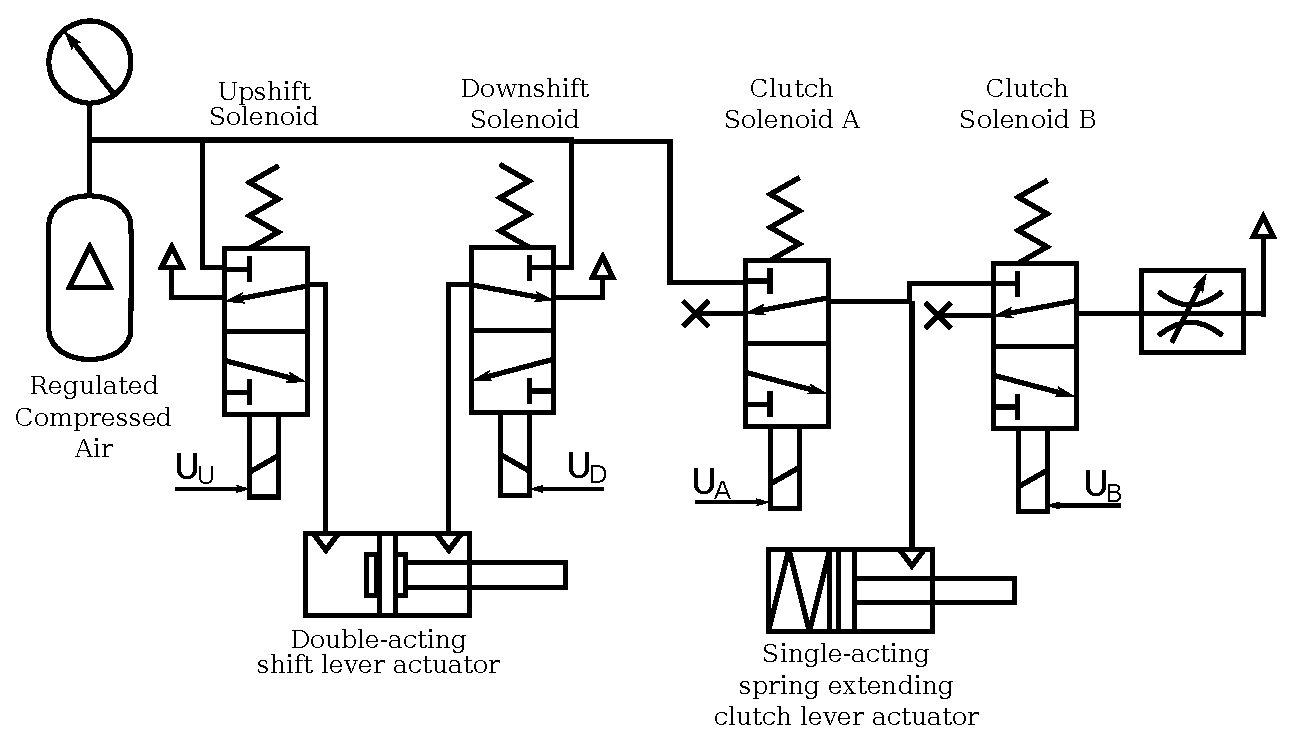
\includegraphics[scale=0.5]{design/figures/pneumatics}
	\caption{Transmission control pneumatics design.}
	\label{fig:pneumatics_design}
\end{figure}

\subsection{Clutch Lever Actuation}
\nomenclature{PWM}{Pulse Width Modulation}
\nomenclature{$U_U$, $U_D$}{Output signals from the transmission controller to the upshift and downshift solenoids.}
\nomenclature{$U_A$, $U_B$}{Pulse width modulated output signals from the transmission controller to clutch solenoids A and B.}

The three approaches described in \cite{pneumatic_actuator, adaptive_pneumatic, accurate_position} considered the possibility of a highly dynamic load on the actuator. The load seen by the clutch actuator is far more predictable than the loads they expected and is only uni-directional. Since the vehicle is only equipped with a limited supply of air, conservation is a concern. Taking these factors into account, a single-acting cylinder with a return spring is specified for the clutch, and we propose a new valving scheme that allows a degree of controllability over actuator while conserving as much air as possible.

The cylinder visible on the right of Fig. \ref{fig:pneumatics_design}, actuates the clutch lever. Precise control of the clutch is accomplished with fast solenoid valves \emph{Clutch Solenoid A} and \emph{Clutch Solenoid B}. These valves are signalled with \emph{pulse width modulated} (PWM) signals, which modulate the average mass air flow rate into and out separately of the cylinder. Positional feedback for the clutch cylinder is provided by a combination of an internal magnet on the piston in the cylinder and a magnetic sensing membrane potentiometer.

Both clutch solenoids are shown as 3-way (with exhaust ports) valves in Fig. \ref{fig:pneumatics_design}, but the valves are used in a 2-way configuration with the exhaust ports plugged.  This results in the following operation:

\begin{enumerate}
  \item When the pulse width modulated control signal $U_A$ to Clutch Solenoid A is non-zero, the valve will open, and air will flow into the cylinder at a rate proportional to the duty cycle, disengaging the clutch.
  \item When pulses no longer arrive at Clutch Solenoid A (or the duty cycle of $U_A$ approaches 0), the valve remains closed, and any air in the cylinder is trapped. The clutch maintains is position.
  \item When the pulse width modulated control signal $U_B$ to Clutch Solenoid B is non-zero, the valve will open, and any pressure differential between the cylinder and atmosphere will cause air to flow out of the cylinder to atmosphere at a rate proportional to the duty cycle. The clutch springs and the cylinders' internal spring work to return the actuator position to rest, and the clutch engages.
\end{enumerate}

An additional adjustable flow rate control valve (visible on the far right in Fig. \ref{fig:pneumatics_design}) was added to the design to allow additional tuning for during clutch engagement. The electro-pneumatic actuation system meets the controllability requirements outlined in \ref{sec:goals_transmission} when coupled with the transmission controller on the engine and transmission module. No air is wasted in disengaging the clutch and holding the position because the fill and exhaust operations are separately controlled with two valves.

\subsection{Shift Lever Actuation}

The shift lever does not require the same level of control as the clutch, and as such the design of the valving has not changed over previous implementations. Two binary valves are used with a dual-acting cylinder. The first actuator (visible on the left of Fig. \ref{fig:pneumatics_design}) actuates the shift lever between 3 different positions: up-shift, down-shift, and rest-state. The transmission spring-loads the lever to automatically return to the rest-state, which is half-way through the actuator stroke. Applying pressure to one port will pull the lever up, and applying pressure to the other port will pull the lever down.

Current gear position is determined with a potentiometer that is mechanically linked to the shift drum. Control and timing are generated by the engine and transmission controller.

\section{Engine and Transmission Module}

The engine and transmission module provides optimized selection of the variable-length intake, changes gears at the driver's request without requiring manual clutching, and provides transmission features that make driving easier. Figure \ref{fig:design_engine_overview} shows an overview of the engine and transmission module and it's interactions with the environment.

\begin{figure}[H]
	\centering
	\input{design/figures/engine_overview_block}
	\caption{An overview of the engine and transmission module and it's environmental interactions.}
	\label{fig:design_engine_overview_block}
\end{figure}

The intake runner position is mechanically actuated with a \emph{servo motor}. The module generates the control signals required by electro-pneumatic system to actuate both the clutch and shift levers. The ECU interfaces with the module both directly through discrete inputs and through the CAN bus.

\subsection{Processes}

The major processes of the engine and transmission module are \emph{up-shifting}, \emph{down-shifting}, and \emph{neutral find}. They are described at a high level using flow charts. Requests to perform these processes are broadcast over the network from the driver interface. The module listens for these requests and executes the correct process accordingly.

\subsubsection{Up-shifting}

The up-shift procedure is described in \ref{fig:transmission_upshift_flow}. Up-shifting does not require disengaging the clutch, merely a small decrease in engine RPM. The ECU provides a shift-cut feature to cut spark to the engine during a shift operation to avoid the driver having to manually modulate the throttle during a shift.

\begin{figure}[H]
	\centering
	\begin{tikzpicture}[auto, node distance=2cm, draw=black!70, >=stealth', font=\scriptsize]
  \node[start, text width=1.2cm] (start) {Upshift Request};
  \node [decision, right of=start, text width=1cm, inner sep=0pt, node distance=2.5cm] (at_top) {Top\\gear?};
  \node [end, below of=at_top] (done) {Done};
  \node [block, right of=at_top, text width=1.5cm, node distance=2.5cm] (shiftcut) {Enable shiftcut};

  \node [block, right of=shiftcut, text width=1.5cm, node distance=2.5cm] (wait_shiftcut) {Wait for RPM drop below $RPM^{TH}_{cut}$};
  \node [block, right of=wait_shiftcut, text width=1.5cm, node distance=2.5cm] (upshift) {Engage upshift solenoid};
  \node [block, right of=upshift, text width=1.5cm, node distance=2.5cm] (wait_upshift) {Wait for shift feedback};
  \node [block, below of=wait_upshift, text width=1.5cm] (upshift_off) {Disengage upshift solenoid};
  \node [block, left of=upshift_off, text width=1.5cm, node distance=2.5cm] (shiftcut_off) {Disable shiftcut};

  \draw [->, thick] (start) -- (at_top);
  \draw [->, thick] (at_top) -- node[]{yes} (done);
  \draw [->, thick] (at_top) -- node[]{no} (shiftcut);

  \draw [->, thick] (shiftcut) -- (wait_shiftcut);
  \draw [->, thick] (wait_shiftcut) -- (upshift);
  \draw [->, thick] (upshift) -- (wait_upshift);
  \draw [->, thick] (wait_upshift) -- (upshift_off);
  \draw [->, thick] (upshift_off) -- (shiftcut_off);
  \draw [->, thick] (shiftcut_off) -- (done);
\end{tikzpicture}

	\caption{Transmission upshift procedure.}
	\label{fig:transmission_upshift_flow}
\end{figure}

The up-shift process depends upon engine RPM and gear position, both of which are provided by the ECU. The shift-cut feature is engaged on the ECU to drop the engine RPM by a small amount known as the cut RPM threshold, or $RPM^{TH}_{cut}$. The exact value of $RPM^{TH}_{cut}$ can be tuned on the ECU. Once the RPM reaches the cut threshold, the upshift solenoid is engaged, which actuates the pneumatics to push the shift lever. Once the module receives notification that the current gear has incremented, the pneumatics are relaxed, and shift cut feature is disengaged.

\nomenclature{$RPM^{TH}_{cut}$}{The threshold RPM is expected to drop when shift-cut is engaged for no-lift up-shifting.}

\subsubsection{Down-shifting}

The down-shift procedure is described in \ref{fig:transmission_downshift_flow}. Unlike up-shifting, down-shifting requires disengaging the clutch, merely a small decrease in engine RPM. The ECU provides a shift-cut feature to cut spark to the engine during a shift operation to avoid the driver having to manually modulate the throttle during a shift.

When the Transmission Manager receives a down-shift request over the network, similar to the up-shift request handling, it creates asynchronous events in the Event Scheduler to respond to the request. Figure \ref{fig:transmission_downshift_flow} shows the flow chart of the downshift procedure. Clutch engagement and disengagement is handled asynchronously by the Clutch Controller. The downshift procedure differs from the upshift procedure in that the downshift requires use of the clutch, as well as two asynchronous incoming events from the driver:

\begin{enumerate}
  \item The original downshift request, when the driver pulls and holds the downshift paddle on the steering wheel, and
  \item a clutch engagement request, issued when the driver releases the downshift paddle.
\end{enumerate}

Adding this extra clutch engagement request allows the driver to delay re-engagement of the clutch so that they can blip the throttle to avoid engine compression and the possibility of a spinout when the clutch plates re-engage (this was explained in Sec. \ref{sec:background_transmission}.)

Additionally, a minimum clutch disengagement time $t^{clutch}_{min}$ is observed (another tunable parameter) in the event the driver pulls the paddle and releases it without any delay.

\nomenclature{$t^{clutch}_{min}$}{Minimum clutch disengagement time during a downshift request.}

\begin{figure}[H]
\centering
\begin{tikzpicture}[auto, node distance=2cm, draw=black!70, >=stealth', font=\scriptsize]
  \node[start, text width=1.4cm] (start) {Downshift Request};
  \node [decision, right of=start, text width=1cm, inner sep=0pt, node distance=2.5cm] (in_neutral) {Neutral?};
  \node [end, below of=in_neutral] (done) {Done};
  \node [block, right of=in_neutral, text width=1.5cm, node distance=2.5cm] (clutchin) {Disengage clutch};

  \node [block, right of=clutchin, text width=1.5cm, node distance=2.5cm] (downshift) {Engage downshift solenoid};
  \node [block, right of=downshift, text width=1.5cm, node distance=2.5cm] (wait_downshift) {Wait for shift feedback};
  \node [block, right of=wait_downshift, text width=1.5cm, node distance=2.5cm] (downshift_off) {Disengage downshift solenoid};
  \node [block, below of=downshift_off, text width=1.5cm] (wait_clutchin) {Wait for clutch-in request};
  \node [block, left of=wait_clutchin, text width=1.5cm, node distance=2.5cm] (clutchout) {Engage clutch};

  \draw [->, thick] (start) -- (in_neutral);
  \draw [->, thick] (in_neutral) -- node[]{yes} (done);
  \draw [->, thick] (in_neutral) -- node[]{no} (clutchin);

  \draw [->, thick] (clutchin) -- (downshift);
  \draw [->, thick] (downshift) -- (wait_downshift);
  \draw [->, thick] (wait_downshift) -- (downshift_off);
  \draw [->, thick] (downshift_off) -- (wait_clutchin);
  \draw [->, thick] (wait_clutchin) -- (clutchout);

  \draw [->, thick] (clutchout) -- (done);
\end{tikzpicture}

\caption{Transmission downshift procedure.}
\label{fig:transmission_downshift_flow}
\end{figure}

\subsubsection{Variable Intake}

\subsubsection{Gear Selection \label{sec:design_engine_transmission_gear_selection}}


\subsubsection{Advanced Transmission Features}

\begin{description}

\item[Auto Upshift Feature]

This feature of the engine module is aimed primarily at improving performance in the acceleration event. Based on known torque curves, a table of optimal shift points in the RPM range is developed. As the engine reaches the top RPM for a given gear, the engine module will automatically upshift to the next gear, without any driver input. All the driver needs to do is maintain full throttle, and hold on.

\item[Launch]
Full-throttle launch uses an important feature of the ECU called launch control. From a stand-still, the slip ratio of the driven wheels to the non-driven wheels is monitored, and the engine output power is reduced until the ratio reaches 1:1. Drivers use this feature by maintaining full-throttle at the starting line while holding the brake pedal. As soon as the brake pedal is released, the the engine module will release the clutch in a controlled manner in an attempt to get the best possible acceleration.

\item[Crawl]
Part-throttle launch is a feature designed to mimic an automatic transmission. By controlling the clutch position, and thereby modulating the amount of torque transferred to the wheels for a short period of time, the car can be made to creep slowly from a standstill. This will be used when driving up to the starting line of various dynamic events.

\item[Neutral Find]
As drivers come in to the pits from driving the course, a useful feature is the ability for the car to shift the transmission back into neutral to avoid stalling the car. The neutral find feature will automatically downshift the transmission repeatedly until it finds neutral.

\end{description}


\subsection{Software}

Software overview diagram


\subsubsection{Transmission Manager}

Listens to transmission requests from the driver over the network.

Uses the event scheduler to sequence the complex series of actuation vectors required by upshifting and downshifting.

Implement the PID feedback controller used to actuate the pneumatic system.

Interacts with the PWM generator to create the control signals required to actuate the pneumatic system.


\subsubsection{Intake Manager}

Continously monitor engine RPM and throttle position through messages from the ECU.

Will adjust intake runner length based on a functional map of RPM and throttle position.

Use hysterisis to avoid instability.

Map will be generated through dynometer testing.


\subsubsection{Starter Manager}

Listen for driver requests to start the engine.

Provide a means of one-touch starting -- sequences the actual starting of the engine through the solenoid driver. 


\subsubsection{Event Scheduler}

Allow for complex sequencing of events in time.

Controllers may schedule new events to occur at various points in time.

Scheduler will continuously update the schedule and signal the main control loop to execute events that are now current.


\subsubsection{CAN Interface}

Provide a means of interfacing with the physical bus. 

Allow direction of particular messages to particular modules.


\subsubsection{PWM Generator}

Generate PWM signals of at least 20 Hz with a resolution of 1\% duty
cycle.

Two-channel design


\subsubsection{Main Control Loop}

Initializes the system and brings into a known state.

Waits for pending events to be executed and executes them.

Monitor for system faults and react accordingly.


\subsection{Hardware}

Show system hardware diagram


\subsubsection{Microcontroller}

Execute system control software.

In-circuit programmable and debuggable.

Has built-in CAN controller.

Has built-in RAM and ROM as well as EEPROM for holding configuration parameters.


\subsubsection{CAN transceiver}

Interface module with the CAN bus.

Be capable of terminating the bus.


\subsubsection{High current solenoid drivers}


Controlling pneumatic solenoid valves (4)

Controlling starter solenoid


\subsubsection{I/O lines to the ECU}

The engine and transmission module has a several CMOS-level outputs to discrete control pins on the ECU:

\begin{itemize}
  \item A line to the launch control pin, which when toggled enables and disables the launch control feature,
  \item A line to the shift cut pin, which when held high enables shift cut, decreasing engine power to allow for an upshift,
  \item A line to the traction cut percent pin, which is a \unit{0-5}{\volt} level signalled input changing the amount of acceptable wheel slip before traction control cuts in.
  \item A line to the traction control on/off pin, which toggles the traction control feature,
  \item A line to the traction control wet/dry pin, which swaps between two traction control presets.
\end{itemize}

The outputs of these lines are controlled in the system software through the event scheduler. 
\section{Braking Module\label{sec:Braking-Module-Design}}

The braking module adjusts the brake bias electronically as requested by the driver. It also provides the ability to calibrate itself to account for mechanical wear and a degree of component tolerance that may cause unwanted rotation of the balance bar. Figure \ref{fig:design_brake_overview_block} shows an overview of the braking module and it's interactions with the environment. 

\begin{figure}[H]
\centering
\begin{tikzpicture}[auto, node distance=2cm, draw=black!70, >=stealth', font=\footnotesize]
  \node [block, minimum width=2cm, inner xsep=0] (pressure1) {Front Pressure Sensor};
  \node [block, minimum width=2cm, inner xsep=0, right of=pressure1, node distance=4cm] (pressure2) {Front Pressure Sensor};

  \node [block, blue shiny, minimum width=6cm, text width=4cm, below of=pressure1, right=-1cm, node distance=1.5cm] (module) {Braking Module};

  \node [block, below of=pressure1, right=-1cm, node distance=3cm, text width=1.1cm] (eot1) {Left EOT Switch};
  \node [block, below of=pressure2, left=-1cm, node distance=3cm, text width=1.1cm] (eot2) {Right EOT Switch};

  \node at ($(eot1)!0.5!(eot2)$) [red shiny, circle, label={[text width=1.5cm, rotate=90, below=5pt, left=10pt]below right:Stepper Motor}] (motor) {M};

  \node [rectangle, below of=motor, minimum width=2cm, label=below:Bias Bar, pattern=north east lines, node distance=1cm] (bias) {};

  \draw [->, thick] (pressure1.south) to ($(module.north west)!(pressure1.south)!(module.north east)$);
  \draw [->, thick] (pressure2.south) to ($(module.north west)!(pressure2.south)!(module.north east)$);

  \draw [->, thick] (eot1.north) to ($(module.south west)!(eot1.north)!(module.south east)$);
  \draw [->, thick] (eot2.north) to ($(module.south west)!(eot2.north)!(module.south east)$);

  \draw [<-, thick] (motor.north) to ($(module.south west)!(motor.north)!(module.south east)$);
  \draw [->, thick, dashed] (motor.south) to ($(bias.north west)!(motor.south)!(bias.north east)$);

  \draw [->, thick, dashed] (bias) -| (eot1);
  \draw [->, thick, dashed] (bias) -| (eot2);

  %%% CAN Bus

  \node [bus, name=can1, right of=module, label={[rotate=90, left=0.75cm]below right:CAN Bus}, node distance=3.5cm] {CAN Bus};
  \node [bus, name=can2, below of=can1, node distance=1cm] {};
  \node [bus, name=can3, above of=can1, node distance=1cm] {};

  \draw [<->, thick] (module) to (can1);
  \draw [-, line width=3pt] (can1) -- (can2);
  \draw [-, line width=3pt] (can1) -- (can3);

  %%% Legend

  \draw [->, thick] ($(eot2.east)+(2cm,0cm)$) -- ++(0.5cm,0) node [label={[font=\tiny]below:Electrical}] {} -- ++(0.5cm,0);
  \draw [->, thick, dashed] ($(eot2.south east)+(2cm,0cm)$) -- ++(0.5cm,0) node [label={[font=\tiny]below:Mechanical}] {} -- ++ (0.5cm,0);
\end{tikzpicture}
\caption{Overview of the braking module and it's environment.}
\label{fig:design_brake_overview_block}
\end{figure}

A \emph{stepper motor} is connected to the balance bar and used to rotate it to the desired position. The motor is bi-directional and can provide the resolution required to allow a 0.5\% bias ratio adjustment. Two \emph{end-of-travel switches} are used to determine when the balance bar is at it's end of travel. \emph{Pressure sensors} on the front and rear braking cylinders are used to determine the current pressure in each system. These components were chosen as part of the mechanical design of the brake pedal assembly by another team member. The actual choice of stepper motor has yet to be determined.

\subsection{Driver-Initiated Processes \label{sec:braking_processes}}

The major processes of the braking module are \emph{brake bias adjustment}, \emph{brake bias calibration}, and \emph{pressure calibration}. Requests to perform either of the processes are broadcast over the network from the driver interface. The module listens for these requests and executes the correct process accordingly. 

\subsubsection{Brake Bias Adjustment}

The brake bias adjustment procedure is shown in Fig. \ref{fig:design-braking-bias-adjustment}. The module performs a series of safety checks before rotating the balance bar to adjust the relative force distribution between the two brake master cylinders.

\begin{figure}[H]
	\centering
	\begin{tikzpicture}[auto, node distance=2cm, draw=black!70, >=stealth', font=\scriptsize]
  \node [start] (start) {Start};
  \node [decision, right of=start, text width=1cm, inner sep=0pt] (brakes_on) {Safe to\\adjust?};
  \node [decision, right of=brakes_on, text width=1cm, inner sep=0pt, node distance=2.5cm] (valid_bias) {Valid bias?};
  \node [end, below of=start, node distance=1cm] (abort) {Abort};

  \node [block, right of=valid_bias, text width=1.5cm, inner xsep=0pt, node distance=2.5cm] (calc) {Calculate offset steps};
  \node [block, right of=calc, text width=1.5cm, inner xsep=0pt, node distance=2.5cm] (step) {Step by offset};
  \node [block, right of=step, text width=1cm, inner xsep=0pt] (store) {Store new offset};
  \node [end, right of=store] (done) {Done};

  \draw [->, thick] (start) to (brakes_on);
  \draw [->, thick] (brakes_on) to (valid_bias);
  \draw [->, thick] (brakes_on.south) |- node[below]{yes} (abort);
  \draw [->, thick] (valid_bias.south) |- node[below]{no} (abort);
  \draw [->, thick] (brakes_on) to node[above]{no} (valid_bias);
  \draw [->, thick] (valid_bias) to node[above]{yes} (calc);
  \draw [->, thick] (calc) to (step);
  \draw [->, thick] (step) to (store);
  \draw [->, thick] (store) to (done);
\end{tikzpicture}

	\caption{Flow-chart for the brake bias adjustment procedure.}
	\label{fig:design-braking-bias-adjustment}
\end{figure}

Of prime importance is that the vehicle is not in motion and the brakes are not engaged while the adjustment is underway. The desired bias ratio is also validated before any adjustment is attempted. If the vehicle is stopped, the brakes are not engaged, and the request is valid, the adjustment may proceed. The module calculates the number of steps required to move from the current position to the desired offset and signals the motor to advance this many steps in the correct direction.

\subsubsection{Brake Bias Calibration}

A flow-chart of the brake bias calibration procedure is shown in Fig. \ref{fig:brake_bias_calibration_flow}. By recording the number of steps it takes to rotate the balance bar from through it's range of motion, we can determine the correct centre point for the bias bar. 

\begin{figure}[H]
	\centering
	\begin{tikzpicture}[auto, node distance=2cm, draw=black!70, >=stealth', font=\scriptsize]
  \node [start] (start) {Start};

  \node [block, right of=start, text width=1cm, inner xsep=0pt] (step_left) {Step Left};
  \node [decision, right of=step_left, text width=1.0cm, inner sep=0pt] (at_left) {At leftend?};

  \node [block, right of=at_left, text width=1cm, inner xsep=0pt] (step_right) {Step Right};
  \node [block, right of=step_right, text width=1cm, inner xsep=2pt] (count) {Add to count};
  \node [decision, right of=count, text width=1cm, inner sep=0pt] (at_right) {At rightend?};

  \node [block, below of=at_right, text width=2cm, inner xsep=2pt, node distance=2.5cm] (adjust) {Adjust bias to old value};
  \node [block, left of=adjust, text width=1.5cm, inner xsep=2pt, node distance=3cm] (store) {Store calibration};
  \node [end, left of=store, node distance=7cm] (end) {Done};

  \draw [->, thick] (start) to node[coordinate, name=x1]{} (step_left);
  \draw [->, thick] (step_left) to (at_left);
  \draw [->, thick] (at_left.south) -- ++(0,-0.25) node[below]{no} -| (x1);
  \draw [->, thick] (at_left.east) to node[name=x2]{yes} (step_right);
  \draw [->, thick] (step_right) to (count);
  \draw [->, thick] (count) to (at_right);
  \draw [->, thick] (at_right.south) -- ++(0,-0.25) node[below]{no} -| (x2);

  \draw [->, thick] (at_right.east) -- ++(0.5,0) node[above]{yes} |- (adjust);
  \draw [->, thick] (adjust) to (store);
  \draw [->, thick] (store) to (end);
\end{tikzpicture}

	\caption{Flow-chart for the brake bias calibration procedure.}
	\label{fig:brake_bias_calibration_flow}
\end{figure}

The first step in calibrating the brake bias is to rotate the balance bar to it's leftmost point of travel, where it pushes on the left end-of-travel switch. This signals the module that the leftmost extreme has been reached. Next, the balance bar is rotated to it's rightmost point of travel, until it pushes on the right end-of-travel switch. The module counts the steps required to travel through it's range of motion and saves the count in non-volatile parameter storage. Finally, the brake bias ratio is adjusted back to it's previous value.

\subsubsection{Pressure Calibration}

The pressure sensor calibration routine is outlined in Fig. \ref{fig:brake_pressure_calibration_flow}. The module keeps track of the minimum and maximum pressures that will be present in both the front and rear systems. This allows it to determine when the brakes are engaged, and to what extent.

\begin{figure}[H]
	\centering
	\begin{tikzpicture}[auto, node distance=2cm, draw=black!70, >=stealth', font=\scriptsize]
  \node [start] (start) {Start};
  \node [decision, right of=start, right=0cm, text width=1.4cm, inner sep=0pt] (min) {Min Applied?};
  \node [block, right of=min, text width=2cm, inner xsep=0pt, node distance=3cm] (sample1) {Sample Pressures};
  \node [decision, right of=sample1, right=0cm, text width=1.4cm, inner sep=0pt] (max) {Max Applied?};
  \node [block, right of=max, text width=2cm, inner xsep=0pt, node distance=3cm] (sample2) {Sample Pressures};

  \node [decision, below of=sample2, text width=1.4cm, inner sep=0pt, node distance=2.5cm] (valid) {Valid samples?};
  \node [block, left of=valid, text width=1.5cm, inner xsep=2pt, node distance=3cm] (save) {Save Calibration};

  \node [end, below of=save] (success) {Success};
  \node [end, below of=valid] (fail) {Fail};

  \draw [->, thick] (start) -- ($(start.east)!0.5!(min.west)$) node[name=x1,coordinate]{} -- (min);
  \draw [->, thick] (min.south) -- ++(0,-0.25cm) node[below]{no} -| (x1);
  \draw [->, thick] (min) to node [] {yes} (sample1);

  \draw [->, thick] (sample1) to node [name=x2]{} (max);
  \draw [->, thick] (max.south) -- ++(0,-0.25cm) node[below]{no} -| (x2);
  \draw [->, thick] (max) to node [] {yes} (sample2);

  \draw [->, thick] (sample2) to (valid);
  \draw [->, thick] (valid) to node [above] {yes} (save);

  \draw [->, thick] (save) to (success);
  \draw [->, thick] (valid.south) to node [] {no} (fail);

\end{tikzpicture}
	\caption{Flow-chart for the brake pressure calibration sequence.}
	\label{fig:brake_pressure_calibration_flow}
\end{figure}

The first step of pressure calibration is to ask the driver to apply minimum pressure. The brake module signals the driver interface to request the driver take their foot off the brake. Once done, the driver interface signals the brake module that minimum pressure has been applied. The brake module then samples the current pressure in both systems. This procedure is repeated for maximum pressure by asking the driver to push on the brake as hard as possible. If the samples are valid, meaning the minimum pressures are less than the maximum pressures and there is a minimum pressure difference between fully-released and fully-applied, the sampled pressures are stored in non-volatile memory.

\subsection{Hardware}

A high-level overview of the module's hardware design is shown in Fig. \ref{fig:brake_hardware_design_block}. Like the other modules, the heart of the brake module is a micro-controller that runs the software necessary to implement all of the required features. 

\begin{figure}[H]
\centering
\begin{tikzpicture}[auto, node distance=2cm, draw=black!70, >=stealth']
%  \draw[help lines] (-3,-5) grid (8,2);

  %%% Pressure Sensors
  \node [block, name=pressure1, font=\scriptsize, text width=1.5cm, inner xsep=0] {Front Pressure Sensor};
  \node [block, name=pressure2, right of=pressure1, font=\scriptsize, text width=1.5cm, inner xsep=0] {Rear Pressure Sensor};

  %%% Balance bar and EOT switches
  \node [block, name=eot1, right of=pressure2, font=\scriptsize, text width=1.5cm, node distance=3cm] {Left EOT Switch};
  \node [block, name=balance, right of=eot1, font=\scriptsize, text width=1.25cm, inner xsep=0] {Balance Bar};
  \node [block, name=eot2, right of=balance, font=\scriptsize, text width=1.5cm] {Right EOT Switch};

  \node [red shiny, circle, below of=balance, name=motor, node distance=1cm, inner sep=1pt] {M};
  \node [block, below of=motor, node distance=1cm, text width=1.5cm, font=\scriptsize] (driver) {Stepper Driver};

  \draw [->, dashed, thick] (balance) -- (eot1);
  \draw [->, dashed, thick] (balance) -- (eot2);
  \draw [->, dashed, thick] (motor) -- (balance);
  \draw [->, thick] (driver) -- (motor);

  \node [block, name=adc1, below of=pressure1, text width=1.5cm] {ADC};
  \node [block, name=adc2, below of=pressure2, text width=1.5cm] {ADC};

  %%% Microcontroller block
  \path ($(adc1.south west)+(0,-1cm)$) node (mu1) {};
  \path ($(adc1.south west -| eot2.south east) + (0,-1cm)$) node (mu2) {};

  \node [block, name=micro, fit=(mu1) (mu2), inner xsep=0, minimum height=1cm] {Microcontroller};

  \draw [->, thick] (pressure1) to (adc1);
  \draw [->, thick] (pressure2) to (adc2);
  \draw [->, thick] (adc1.south) -- ($(micro.north west)!(adc1.south)!(micro.north east)$);
  \draw [->, thick] (adc2.south) -- ($(micro.north west)!(adc2.south)!(micro.north east)$);

  \draw [->, thick] (eot1.south) -- ($(micro.north west)!(eot1.south)!(micro.north east)$);
  \draw [->, thick] (eot2.south) -- ($(micro.north west)!(eot2.south)!(micro.north east)$);

  \draw [<-, thick] (driver.south) -- ($(micro.north west)!(driver.south)!(micro.north east)$);

  %%% CAN Bus

  \node at ($(micro.east)+(2cm,0)$) [block, name=can, node distance=2cm, inner xsep=2pt] {CAN Transceiver};

  \draw [<->, thick] (micro) to (can);

  \node [bus, name=can1, above of=can, label=above:CAN Bus, node distance=2.5cm] {CAN Bus};
  \node [bus, name=can2, left of=can1, node distance=1cm] {};
  \node [bus, name=can3, right of=can1, node distance=1cm] {};

  \draw [-, line width=3pt] (can) -- (can1);
  \draw [-, line width=3pt] (can1) -- (can2);
  \draw [-, line width=3pt] (can1) -- (can3);

  %%% Background

  \begin{pgfonlayer}{background}
    \path (adc1.north west)+(-0.3,0.3) node (a) {};
    \path (can.south east)+(+0.2,-0.2) node (b) {};
    \path[module] (a) rectangle (b);
  \end{pgfonlayer}

  %%% Legend

  \draw [->, thick] ($(micro.south west)+(0.5cm,-0.5cm)$) -- ++(0.5cm,0) node [label={[font=\tiny]below:Electrical}] {} -- ++(0.5cm,0);
  \draw [->, thick, dashed] ($(micro.south west)+(2cm,-0.5cm)$) -- ++(0.5cm,0) node [label={[font=\tiny]below:Mechanical}] {} -- ++ (0.5cm,0);
\end{tikzpicture}

\caption{Block diagram of the braking module hardware.}
\label{fig:brake_hardware_design_block}
\end{figure}

The module communicates over the bus using a CAN transceiver. A pair of analog-to-digital converters (similar to those used in the engine and transmission module) sample the brake pressure sensors. Unique to the brake module is a \emph{stepper motor driver} that provides the signals necessary to drive the stepper motor connected to the balance bar. The micro-controller interfaces to the end-of-travel switches without any extra hardware.

\subsubsection{Stepper Motor Driver}

The stepper motor driver generates the signals required to drive the stepper motor connected to the balance bar. It must be capable of  driving a bi-polar stepper motor in the clockwise or counter-clockwise direction. It must also supply enough current to generate the torque required to spin the balance bar, which is approximately\footnote{This figure was supplied by the team member responsible for the braking pedal assembly.} \unit{150}{mA}.

\subsubsection{Analogue-to-Digital Converters (ADC)}

The ADCs sample the output voltage from pressure sensors attached to the front and rear brake master cylinders. The output voltage of the particular sensors used is \unit{0-5}{\volt}, corresponding to \unit{0-10}{\mega\pascal}. The expected maximum brake pressure is somewhere around \unit{7}{\mega\pascal}. To achieve resolution of \unit{10}{\kilo\pascal}, a 10-bit ADC is sufficient. The pressure values are sampled at \unit{10}{\hertz}.

\subsubsection{End-of-Travel Sensing Switches}

Two end-of-travel switches are tripped whenever the balance bar reaches it's leftmost or rightmost extremes. The switches are normally high-impedance, and become switched to ground. The micro-controller should have GPIO pins with weak internal pull-up resistors to detect the state of the switches.

\subsection{Software}

A block-diagram overview of the software design is shown in Fig. \ref{fig:brake_software_design_block}. The functionality of the system is separated into a \emph{bias manager} and a \emph{pressure manager}. Like the engine and transmission module, the managers interact with a set of hardware abstraction interfaces to perform their tasks, and the entire process is overseen by a \emph{module coordinator}.

\begin{figure}[H]
	\centering
	\tikzstyle{big arrow} = [>=latex, line width=4pt, gray]

\begin{tikzpicture}[auto, node distance=2cm, draw=black!70, >=stealth']
  \node [block, minimum width=2cm, inner xsep=0] (stepper) {Stepper Interface};
  \node [block, minimum width=2cm, inner xsep=0, right of=stepper, node distance=3cm] (io) {I/O Interface};

  \node [block, grey shiny, minimum width=5cm, inner xsep=0, below of=stepper, right=-1cm, text width=5cm, node distance=2cm] (bias_manager) {Bias Manager};

  \node [block, minimum width=2cm, inner xsep=0, below of=stepper, node distance=4cm] (can) {CAN Interface};
  \node [block, minimum width=2.2cm, inner xsep=0, below of=io, node distance=4cm] (nv) {NV Storage Interface};
  \node [block, blue shiny, minimum width=2.5cm, text width=2.2cm, inner xsep=0, right of=nv, node distance=3cm] (coordinator) {Module Coordinator};
  \node [block, minimum width=2cm, inner xsep=0, left of=can, node distance=3cm] (adc) {ADC Interface};

  \node [block, grey shiny, minimum width=5cm, inner xsep=0, below of=can, right=-1cm, text width=5cm, node distance=2cm] (pressure_manager) {Pressure Manager};

  \draw [<-, big arrow] (stepper.south) -- ($(bias_manager.north west)!(stepper.south)!(bias_manager.north east)$);
  \draw [->, big arrow] (io.south) -- ($(bias_manager.north west)!(io.south)!(bias_manager.north east)$);

  \draw [<->, big arrow] (can.north) -- ($(bias_manager.south west)!(can.north)!(bias_manager.south east)$);
  \draw [<->, big arrow] (nv.north) -- ($(bias_manager.south west)!(nv.north)!(bias_manager.south east)$);

  \draw [<->, big arrow] (can.south) -- ($(pressure_manager.north west)!(can.south)!(pressure_manager.north east)$);
  \draw [<->, big arrow] (nv.south) -- ($(pressure_manager.north west)!(nv.south)!(pressure_manager.north east)$);

  \draw [<->, big arrow] (bias_manager) -| (coordinator);
  \draw [<->, big arrow] (pressure_manager) -| (coordinator);
  \draw [->, big arrow] (adc) |- (pressure_manager);

  \draw [-, thick] ($(coordinator.south)!0.5!(coordinator.south west)$) |- ($(nv.south)!0.5!(nv.south east)+(0,-0.6cm)$) node [name=x, inner sep=0]{};
  \draw [->, thick] (x) -- ($(nv.south)!0.5!(nv.south east)$);
  \draw [->, thick] (x) -| ($(can.south)!0.5!(can.south east)$);

  \draw [-, thick] (adc.east) -| ($(stepper.south west)+(-0.5cm,-0.6cm)$) node [name=x2, inner sep=0]{};
  \draw [->, thick] (x2) -| ($(stepper.south)!0.5!(stepper.south east)$);
  \draw [->, thick] (x2) -| ($(io.south)!0.5!(io.south east)$);
  
\end{tikzpicture}

	\caption{Block diagram of the braking module software.}
	\label{fig:brake_software_design_block}
\end{figure}

Several hardware abstraction interfaces link the external hardware and micro-controller features to the bias and pressure managers. Unique to the braking module is the \emph{stepper motor interface}. The CAN interface is exactly as described earlier, and is not mentioned here.

\subsubsection{Bias Manager}

The bias manager implements the bias adjustment and bias calibration processes. It listens for requests to initiate either process from the network by way of the CAN interface.

When asked to adjust the brake bias, the bias manager coordinates with the pressure manager to determine if the brakes are being applied, and with the engine and transmission controller to determine if the vehicle is in motion. It performs the calculations required to calculate the new bias position, and adjusts the balance bar accordingly by sending motor step commands to the stepper motor interface.

Bias calibration requires similar coordination to ensure a safe operating state. The bias manager again uses the stepper motor interface to move the balance bar between it's extremes. Calibration data is loaded at start-up and stored after calibration in NVRAM by way of the non-volatile storage interface.

\subsubsection{Pressure Manager}

The pressure manager periodically outputs the front and rear brake pressures. It also implements the pressure calibration procedure and listens for calibration requests over the network, similar to the bias manager.

The front and rear pressures are sampled through the ADC interface. The pressure manager uses the CAN interface to output the samples over the network. Current pressure readings are made available to the bias manager to avoid adjusting or calibrating the bias while the brakes are engaged.

The pressure manager communicates with the driver interface through the CAN interface to coordinate the sequence of driver inputs required to calibrate the front and rear brake pressures. Like the pressure manager, calibration data is loaded at start-up and stored after calibration through the non-volatile storage interface.

\subsubsection{Module Coordinator}

Like the module coordinator for the engine and transmission module, the braking module coordinator contains the low-level state machine mechanisms needed by the two managers to transition between their internal states. It keeps track of the current state of the system, and also initializes all of the hardware abstraction interfaces and managers at start-up time. 

\subsubsection{Stepper Motor Interface}

The stepper motor interface takes motor movement commands from the program and converts them into commands for the stepper motor driver. It can direct the stepper motor driver to turn clockwise or counter-clockwise, and move an arbitrary number of steps. 

\subsubsection{GPIO Interface}

The GPIO interface monitors the state of the end-of-travel buttons. It can asynchronously interrupt the program when a change of state occurs. 

\subsubsection{ADC Interface}  

The ADC interface initiates a sampling cycle on either pressure sensor channel. The resulting sample is provided to  the program for further processing. 

\subsubsection{Non-Volatile Storage Interface}

The \emph{non-volatile storage interface} reads and writes calibration data to the non-volatile storage portion of the micro-controller. It is also used to keep track of the current position of the bias bar, so calibration is not required between start-ups.


\section{Telemetry Module\label{sec:Telemetry-Module-Design}}

The \emph{telemetry module} provides a means for multiplexing the ECU and DAQ data streams, and sending them wirelessly to the crew's laptops. The module also decodes data from the DAQ and makes it available over the network to other modules, and injects data from other modules into the DAQ stream. An overview of the telemetry module and its environmental interactions is shown in Fig.\ \ref{fig:design_telemetry_overview_block}.

\begin{figure}[H]
	\centering
	\begin{tikzpicture}[auto, node distance=2cm, draw=black!70, >=stealth']
  \node [block, blue shiny, minimum width=4cm, text width=4cm] (module) {Telemetry Module};
  \node [block, left of=module, node distance=4cm, font=\scriptsize, text width=1.5cm] (modem) {Wireless Modem};
  \node [block, below of=module, left=-2cm, text width=1cm, node distance=1.5cm] (ecu) {ECU};
  \node [block, below of=module, right=-2cm, text width=1cm, node distance=1.5cm] (dac) {DAC};

  \draw [-, thick] (modem.north) \antenna;
  \draw [<->, thick] (modem) -- (module);
  \draw [<->, thick] (ecu) -- ($(module.south west)!(ecu.north)!(module.south east)$);
  \draw [<->, thick] (dac) -- ($(module.south west)!(dac.north)!(module.south east)$);

  \node [bus, right of=ecu] (can1) {};
  \node [bus, above of=can1, node distance=1.5cm] (can2) {};

  \draw [-, line width=3pt] (can1) -- ++(0,-1cm);
  \draw [-, line width=3pt] (can1) -- node[label={[rotate=90]below:CAN Bus}]{} (can2) -- ++(0,1cm);
  \draw [<->, thick] (ecu) -- (can1);
  \draw [<->, thick] (module) -- (can2);
\end{tikzpicture}

	\caption{Overview of the telemetry module and it's environment.}
	\label{fig:design_telemetry_overview_block}
\end{figure}

The vehicle-side of the telemetry system consists of the telemetry module itself, which gathers and multiplexes the data from the ECU and DAQ over their serial links, and the \emph{wireless modem}, which transmits and receives data wirelessly from the remote laptops. The remote-side of the telemetry system consists of an off-the-shelf wireless receiver, which receives the data and makes it available on an RS-232 port on the laptop.

\subsection{ECU Data Channel}

The ECU data channel is illustrated in Fig.\ \ref{fig:ecu_data_channel}. It is a simple bi-directional pass-through channel. The module acts as a router for ECU data. The data stream is not modified in any way. 

\begin{figure}[H]
	\centering
	\begin{tikzpicture}[auto, node distance=2cm, draw=black!70, >=stealth', font=\scriptsize, minimum height=1cm]
  \node [block, text width=1cm] (ecu) {ECU};
  \node [block, right of=ecu, text width=1cm] (packetizer) {MUX};
  \node [block, right of=packetizer, text width=1.25cm] (modem1) {Wireless Modem};
  
  \draw [->, thick] (ecu) -- (packetizer);
  \draw [->, thick] (packetizer) -- (modem1);
  \draw [-, thick] (modem1.east) -- ++(0.5cm,0) \antenna;

  \node [block, right of=modem1, node distance=4cm, text width=1.25cm] (modem2) {Wireless Modem};
  \node [block, right of=modem2, text width=1cm] (laptop) {Laptop};
  \node [block, right of=laptop, text width=1.25cm] (software) {DTAFast Software};
  
  \draw [-, thick] (modem2.west) -- ++(-0.5cm, 0) \antenna;
  \draw [->, thick] (modem2) -- (laptop);
  \draw [->, thick] (laptop) -- (software);

  \draw [-, thick, dashed] ($(modem1)!0.5!(modem2)+(0,1cm)$) -- ++(0,-2cm) node[](x1){};

  \node at (x1) [anchor=east, inner xsep=0.5cm] (vehicle) {Vehicle Side};
  \node at (x1) [anchor=west, inner xsep=0.5cm] (remote) {Remote Side};
\end{tikzpicture}

	\caption{Data flow of the ECU data channel.}
	\label{fig:ecu_data_channel}
\end{figure}

Data originating from the ECU over the serial link is multiplexed onto the wireless modem's data stream. The data is then broadcast over the modem to the laptop, where it is received by the remote wireless modem. The data is then fed to the laptop and eventually the ECU software. Packets originating from the ECU software flow in the opposite direction with a similar process.

\subsection{DAQ Data Channel}

The DAQ data channel is illustrated in Fig.\ \ref{fig:dac_data_channel}. Unlike the ECU data channel, the DAQ data channel is uni-directional, and data is injected and decoded from the data stream.

\begin{figure}[H]
	\centering
	\begin{tikzpicture}[auto, node distance=1.75cm, draw=black!70, >=stealth', font=\scriptsize, minimum height=1cm]
  \node [block, text width=0.75cm] (dac) {DAC};
  \node [block, right of=dac, text width=1.25cm, above=0.25cm] (injector) {Injector};
  \node [block, right of=injector, text width=0.75cm] (mux) {MUX};
  \node [block, right of=mux, text width=1.25cm] (modem1) {Wireless Modem};

  \node [block, right of=dac, text width=1.25cm, below=0.25cm] (decoder) {Decoder};
  \node [cloud, red shiny, inner sep=0cm, right of=decoder, cloud ignores aspect=true, node distance=2cm] (network) {Network};
  
  \draw [->, thick] (dac) -- (injector);
  \draw [->, thick] (dac) -- (decoder);
  \draw [->, thick] (decoder) -- (network);
  \draw [->, thick] (injector) -- (mux);
  \draw [->, thick] (mux) -- (modem1);
  \draw [-, thick] (modem1.east) -- ++(0.5cm,0) \antenna;

  \node [block, right of=modem1, node distance=4cm, text width=1.25cm] (modem2) {Wireless Modem};
  \node [block, right of=modem2, text width=1cm] (laptop) {Laptop};
  \node [block, right of=laptop, text width=1.25cm] (software) {DTAFast Software};
  
  \draw [-, thick] (modem2.west) -- ++(-0.5cm, 0) \antenna;
  \draw [->, thick] (modem2) -- (laptop);
  \draw [->, thick] (laptop) -- (software);

  \draw [-, thick, dashed] ($(modem1)!0.5!(modem2)+(0,1cm)$) -- ++(0,-3cm) node[](x1){};

  \node at (x1) [anchor=east, inner xsep=0.5cm] (vehicle) {Vehicle Side};
  \node at (x1) [anchor=west, inner xsep=0.5cm] (remote) {Remote Side};
\end{tikzpicture}

	\caption{Data flow of the DAQ data channel.}
	\label{fig:dac_data_channel}
\end{figure}

Data originating from the DAQ is routed to the DAQ software in a fashion similar to the ECU data channel. However, the module has the ability to inject data into the stream as it sees fit. This data must be in a format that the DAQ software can understand. As well, data from the DAQ can be decoded and output over the CAN bus to the other modules. 

At the time of writing, the mechanical team has not identified what data they would like injected or decoded from the DAQ. The injection and decoding features remain provisions for future use. Likely applications will be strain gauge data from stress-loaded members like the suspension, and throttle-brake-steering position data to analyze and improve driver performance.

\subsection{Hardware}

A high-level overview of the module's hardware design is shown in Fig.\ \ref{fig:design_telemetry_hardware_block}. Like the other modules, the heart of the brake module is a micro-controller that runs the software necessary to implement all of the required features. 

\begin{figure}[H]
\centering
\begin{tikzpicture}[auto, node distance=2cm, draw=black!70, >=stealth', font=\scriptsize]
  \node [block, minimum width=1cm] (modem) {Wireless Modem};
  \node [block, text width=1cm, below of=modem, node distance=1.25cm] (uart1) {UART};

  \draw [-, thick] (modem.north) \antenna;

  \node [block, right of=modem, minimum width=3cm, node distance=4cm] (rs232) {RS-232 Transceiver};
  \node [block, above of=rs232, left=-1.5cm, text width=1cm, node distance=1.25cm] (ecu) {ECU};
  \node [block, above of=rs232, right=-1.5cm, text width=1cm, node distance=1.25cm] (dac) {DAC};

  \node [block, below of=rs232, left=-1.5cm, text width=1cm, node distance=1.25cm] (uart2) {UART};
  \node [block, below of=rs232, right=-1.5cm, text width=1cm, node distance=1.25cm] (uart3) {UART};

  \draw [->, thick] (dac) -- ($(rs232.north west)!(dac.south)!(rs232.north east)$);
  \draw [<->, thick] (ecu) -- ($(rs232.north west)!(ecu.south)!(rs232.north east)$);

  \draw [<->, thick] (uart2) -- ($(rs232.south west)!(uart2.north)!(rs232.south east)$);
  \draw [<-, thick] (uart3) -- ($(rs232.south west)!(uart3.north)!(rs232.south east)$);

  %%% Microcontroller block
  \path ($(modem.south west |- uart1.south west) + (0,-1.25cm)$) node (mu1) {};
  \path ($(uart2.south east) + (0,-1.25cm)$) node (mu2) {};

  \node [block, fit=(mu1) (mu2), inner xsep=0, minimum height=1cm] (micro) {Microcontroller};

  \draw [<->, thick] (uart2) -- ($(micro.north west)!(uart2.south)!(micro.north east)$);
  \draw [<-, thick] (uart3) -- ($(micro.north west)!(uart3.south)!(micro.north east)$);

  \draw [<->, thick] (modem) -- (uart1);
  \draw [<->, thick] (uart1) -- ($(micro.north west)!(uart1.south)!(micro.north east)$);

  %%% CAN Bus
  \node at ($(micro.east)+(1.5cm,0)$) [block, name=can, inner xsep=2pt] {CAN Transceiver};
  \draw [<->, thick] (micro) to (can);
  \draw [-, line width=3pt] (can.north) |- node[coordinate,label={above:CAN Bus}](can1){} (ecu.east);
  \draw [-, line width=3pt] (can1) -- ++(1cm,0cm);


  \begin{pgfonlayer}{background}
    \path (micro.south west)+(-0.2cm,-0.2cm) node (a) {};
     \path (can.north east |- rs232.north east)+(+0.2cm,0.2cm) node (b) {};
     \path[module] (a) rectangle (b);
  \end{pgfonlayer}
\end{tikzpicture}

\caption{Block diagram of the telemetry module hardware.}
\label{fig:design_telemetry_hardware_block}
\end{figure}

\nomenclature{UART}{Universal Asynchronous Receiver-Transmitter}

The telemetry module shares the same CAN transceiver used by the other modules. Unique to the module are three \emph{high-speed universal asynchronous receiver-transmitter} (UART) devices, a dual-channel \emph{RS-232 transceiver}, and a \emph{wireless modem}. These features are discussed further below.

\subsubsection{High-Speed UARTs}

The function of a UART is to frame data into serial packets for transmission, and to validate and decode received serial packets. The UART consists of a \emph{receiver} portion and a \emph{transmitter} portion. The receiver portion can be fed bits from a serial link, validate the structure of the serial frame, decode the data contained within the frame, and provide it to the micro-controller. Conversely, the transmitter portion can take data from the micro-controller, frame it for serial transmission, and output the bits to a transceiver for transmission.

Three UARTs are required for the telemetry module; one for interfacing with the DAQ, one for interfacing the ECU, and one for interfacing with the wireless modem. 

\subsubsection{RS-232 Transceiver\label{sec:design_telemetry_rs232}}

The RS-232 transceiver converts the logic-level bit stream from the UARTs into serial-level voltages, and visa-versa. The transceiver acts as the bridge between the UARTs and the ECU and DAQ. Two separate receiver/transmitter channels are required, one each for the ECU and DAQ. The wireless modem does not require a transceiver.

\subsubsection{Wireless Modem}

The wireless modem converts a logic-level serial stream from the one of the UARTs into a wireless signal stream, to be broadcast over an antenna and received by paired wireless modems connected to laptops in the pit. 

\subsection{Software}
	
A block-diagram overview of the software design is shown in Fig.\ \ref{fig:design_telemetry_software_block}. Data streams from the ECU and DAQ are dealt with by the \emph{data manager}. The DAQ stream is decoded by the \emph{packet decoder} and modified by the \emph{packet injector}. The wireless link is overseen by the \emph{link manager}. 

\begin{figure}[H]
	\centering
	\tikzstyle{big arrow} = [>=latex, line width=4pt, gray]

\begin{tikzpicture}[auto, node distance=2cm, draw=black!70, >=stealth']
  \node [block, minimum width=4cm, text width=2.5cm] (data_manager) {Data Manager};
  \node [block, text width=1.5cm, below of=data_manager, left=-2cm, font=\scriptsize] (can_interface) {CAN Interface};
  \node [block, minimum width=4cm, text width=2.5cm, below of=data_manager, node distance=4cm] (link_manager) {Link Manager};

  \node [block, minimum width=1.5cm, text width=1.25cm, above of=data_manager, font=\scriptsize, left=-2cm] (decoder) {Packet Decoder};
  \node [block, minimum width=1.5cm, text width=1.25cm, above of=data_manager, font=\scriptsize, right=-2cm] (injector) {Packet Injector};

  \draw [<->, big arrow] (decoder) -- ($(data_manager.north west)!(decoder.south)!(data_manager.north east)$);
  \draw [<->, big arrow] (injector) -- ($(data_manager.north west)!(injector.south)!(data_manager.north east)$);

  \draw [<->, big arrow] (can_interface) -- ($(data_manager.south west)!(can_interface.north)!(data_manager.south east)$);
  \draw [<->, big arrow] (can_interface) -- ($(link_manager.north west)!(can_interface.south)!(link_manager.north east)$);

  \node [block, minimum width=1.5cm, right of=can_interface, font=\scriptsize, node distance=3.5cm] (init) {Module Initializer};
  \node [block, minimum width=1.5cm, above of=init, font=\scriptsize] (uart) {UART Interface};
  \node [block, minimum width=1.5cm, below of=init, font=\scriptsize] (wireless) {Wireless Modem Interface};

  \draw [->, big arrow] (init) -- (can_interface);
  \draw [->, big arrow] (init) -- (uart);
  \draw [->, big arrow] (init) -- (wireless);
  \draw [<->, big arrow] (uart) -- (data_manager);
  \draw [<->, big arrow] (wireless) -- (link_manager);
  
\end{tikzpicture}

	\caption{Block diagram of the telemetry module software.}
	\label{fig:design_telemetry_software_block}
\end{figure}

As is typical with our design, the high-level systems interact with a set of hardware abstraction interfaces to speak with the low-level systems. 

A \emph{module initializer} brings the entire system into a known state. Unlike the other modules, once the system is initialized, all incoming and outgoing data is handled asynchronously. There is no need for intervention from a module coordinator. 

\subsubsection{Data Manager}

The data manager receives new data from the ECU and DAQ, and multiplexes the two streams for transmission over the wireless modem. Incoming data from the ECU and DAQ arrive from the UART interface. DAQ data is merged with any injected packets, and also sent to the decoder for broadcast. The modified DAQ stream is then merged with the ECU stream and packetized and broadcast with the wireless modem interface. Incoming data from the ECU software is directed oppositely from the wireless modem interface to the ECU's UART interface.

\subsubsection{Packet Decoder}
\label{sec:design_telemetry_decoder}

The packet decoder can read the incoming DAQ data stream and rebuild the packets being sent to the DAQ in real-time. The various sensor readings that are captured are then fed to the CAN interface for broadcast to the other modules.

\subsubsection{Packet Injector}
\label{sec:design_telemetry_injector}

The packet injector is the dual of the packet decoder. It can take arbitrary data from other modules over the CAN interface and create new packets to be injected into the DAQ data stream going to the pit laptops. This process is entirely transparent to the DAQ software.

\subsubsection{Link Manager}

The link manager uses the wireless modem interface to configure the modem and monitor the status and strength of the wireless link. The link status is broadcast over the network for the driver interface to relay to the driver. The link manager negotiates automatic channel switching if interference is degrading the link quality.

\subsubsection{Module Initializer}

The module initializer for the telemetry module handles the initial configuration of the module on start-up. It establishes the initial communication between the ECU, DAQ, and modem. 

\subsubsection{UART Interface}

The UART interface allows a data byte to be framed and transmitted over the serial link. It can also alert the program when a new serial frame has been received, and decode the frame for the micro-controller.

\nomenclature{API}{Application Programming Interface}
\subsubsection{Wireless Modem Interface}

The wireless modem has its own \emph{application programming interface} (API) for configuration and data routing data between the two target serial ports on the laptop computer. The wireless modem interface is a window into this API for the telemetry module, so that the features of the modem can be exploited.

\section{Driver Interface Module\label{sec:Driver-Interface-Module}}
\nomenclature{LCD}{Liquid Crystal Display}

In previous years, the team has often been hindered by a lack of direct information from the electronic systems in the car. The driver interface module remedies this by providing information to the driver in real-time, and allows the driver to control aspects of the electronic control systems. The driver module and it's interactions are shown in Fig. \ref{fig:design_interface_overview_block}.

\begin{figure}[H]
	\centering
	\begin{tikzpicture}[auto, node distance=1.25cm, draw=black!70, >=stealth', font=\scriptsize]
  \node [block, blue shiny, text width=5cm] (module) {Driver Interface Module};
  \node [block, above of=module, text width=1cm, right=-2.5cm] (knobs) {Knobs};
  \node [block, above of=module, text width=1.25cm] (buttons) {Buttons};
  \node [block, above of=module, text width=1cm, left=-2.5cm] (paddles) {Paddles};

  \node [block, below of=module, text width=3cm] (panel) {Information Display Panel};

  \draw [->, thick] (knobs.south) -- ($(module.north west)!(knobs.south)!(module.north east)$);
  \draw [->, thick] (buttons.south) -- ($(module.north west)!(buttons.south)!(module.north east)$);
  \draw [->, thick] (paddles.south) -- ($(module.north west)!(paddles.south)!(module.north east)$);

  \draw [->, thick] (module) -- (panel);

  \draw [<->, thick] (module.east) -- ++(1cm,0) node[coordinate,label={[rotate=90]below:CAN Bus}](can){};
  \draw [-, line width=3pt] ($(can)+(0,-1cm)$) -- ++(0,2cm);

  \draw ($(knobs.north west)+(-0.2cm,0.2cm)$) node[coordinate] (x1) {};
  \draw ($(paddles.south east)+(0.2cm,-0.2cm)$) node[coordinate] (x2) {};
  \path [draw, thick, dashed] (x1) rectangle (x2);
  \node at (x1) [anchor=south west] {Driver Controls};
\end{tikzpicture}

	\caption{Overview of the driver interface module and it's interactions.}
	\label{fig:design_interface_overview_block}
\end{figure}

The driver module receives driver input from \emph{driver controls}, which are tactile inputs for adjusting vehicle dynamics. Driver commands are collected through the controls and relayed across the network to the relevant modules. The module communicates with the driver using the \emph{information display panel}, which displays vehicle information on an easy-to-read display mounted in the steering wheel. Diagnostic information from the other modules is received over the network and relayed to the driver through the information display panel. 

\subsection{Vehicle Dynamics Mode (VDM)}
\nomenclature{VDM}{Vehicle Dynamics Mode}

The driver interface system provides a method of quickly modifying several dynamic vehicle parameters quickly and easily. We have called this feature \emph{Vehicle Dynamics Mode} (VDM). 

For example, an acceleration event calls for launch control, auto-upshift, and a heavy forward brake bias. It is possible to enable all of these features in one step by changing the VDM mode to {}``acceleration''. 

When a new mode is selected, all nodes on the network are notified and synchronized to modify their dynamic parameters in accordance with the specific mode. For example, when the  {}``acceleration'' mode is enabled, the engine module will enable launch control and auto-upshift, and the brake controller will modify the brake bias to a pre-set ratio.

\begin{description}
  \item [{Pit Mode}] enables soft-launch driving characteristics that mimic a fully automatic transmission. This makes slowly driving the car forward from a stand-still far easier, and only requires the driver to take their left foot off the brake, and slightly apply the throttle.
  \item [{Acceleration Mode}] puts the vehicle systems into full-performance characteristics. Launch control is activated. The engine module will watch for a launch signal from the driver, and will automatically up-shift based on the engine RPM.
  \item [{Dynamic Mode}] puts the vehicle systems into a mode that is suitable for the autocross, and the endurance race.
\end{description}

Individual VDM parameters can be changed by the driver using the driver controls. Existing presets may be overwritten on demand with the new parameters chosen by the driver.

\subsection{Driver Controls}
\label{sec:interface_controls}

The driver controls consist of adjustment knobs, buttons, and paddle shifters. See table \ref{table:driver_controls} for a description of each.

\begin{table}[H]
\caption{Available driver controls.}
\centering
\begin{tabular}{|c|c|p{8 cm}|}
	\hline 
	Type & Name & Description \\
	\hline
	\hline 
	Knob & VDM & Changes the current VDM setting. \\
	\hline 
	Knob & Option & Changes the currently selected menu option. \\
	\hline
	Knob & Adjust & Adjusts the value associated with the currently selected menu option. \\
	\hline
	Button & Starter & Engages the automatic start sequence if pressed once, or the manual start sequence if held down.\\
	\hline
	Button & Neutral Find & Activates the neutral-find feature. \\
	\hline
	Button & Diagnostics/Save & Pages through diagnostic information if pressed once, or saves the current dynamic settings to the selected VDM if held down.\\		
	\hline 		
	Paddle & Up-Shift & Up-shifts the transmission. \\
	\hline
	Paddle & Down-Shift & When held, disengages the clutch and down-shifts. When released, re-engages the clutch. \\
	\hline
\end{tabular}
\label{table:driver_controls}
\end{table}

\subsection{Diagnostic Information}
\label{sec:interface_diag}

The interface display panel is a large monochrome \emph{Liquid Crystal Display} (LCD) screen, inset in the steering wheel. The panel provides real-time information to the driver regarding all of the electronic systems in the car. Primary information displayed on the panel includes:

\begin{itemize}
\item the selected gear;
\item the active \emph{vehicle dynamics mode} (VDM);
\item the telemetry signal strength;
\item the engine RPM;
\item the vehicle wheel speed; and
\item the status of the launch control feature.
\end{itemize}

The list of available options and the current value for the selected option is displayed on screen when the driver rotates the option dial. After a timeout period, normal real-time information display resumes. 

\subsection{Hardware}

A high-level overview of the module's hardware design is shown in figure \ref{fig:interface_hardware_design_block}. The driver interface module builds on the common architecture present in the other three modules. 

\begin{figure}[H]
\centering
\begin{tikzpicture}[auto, node distance=2cm, draw=black!70, >=stealth']
  \node[block, text width=1.25cm, minimum height=1cm] (lcd) {LCD\\ Module};
  \node[block, right of=lcd, minimum height=1cm, text width=1.15cm] (knobs) {Knobs};
  \node[block, right of=knobs, minimum height=1cm, text width=1.35cm] (buttons) {Buttons};
  \node[block, right of=buttons, text width=1.35cm, minimum height=1cm] (paddles) {Shift\\ Paddles};

  %%% Microcontroller block
  \path ($(lcd.south west) + (0,-1.25cm)$) node[coordinate] (mu1) {};
  \path ($(paddles.south east) + (0,-1.25cm)$) node[coordinate] (mu2) {};

  \node [block, fit=(mu1) (mu2), inner xsep=0, minimum height=1cm] (micro) {Microcontroller};
  \node at ($(micro.east)+(2cm,0)$) [block, text width=2cm] (can_interface) {CAN Transceiver};

  \draw [<->, thick] (lcd.south) -- ($(micro.north west)!(lcd.south)!(micro.north east)$);
  \draw [<->, thick] (knobs.south) -- ($(micro.north west)!(knobs.south)!(micro.north east)$);
  \draw [<->, thick] (buttons.south) -- ($(micro.north west)!(buttons.south)!(micro.north east)$);
  \draw [<-> ,thick] (paddles.south) -- ($(micro.north west)!(paddles.south)!(micro.north east)$);

  \draw [-, line width=3pt] (can_interface.north) -- ++(0, 1cm) node[coordinate,label=above:CAN Bus](x1){} -- ++(1cm,0);
  \draw [-, line width=3pt] (x1) -- ++(-1cm,0);
  

  %%% Background
  \begin{pgfonlayer}{background}
    \path (micro.north west)+(-0.3,0.3) node (a) {};
    \path (can_interface.south east)+(+0.2,-0.2) node (b) {};
    \path[module] (a) rectangle (b);
  \end{pgfonlayer}
\end{tikzpicture}

\caption{A block diagram of interface module hardware.}
\label{fig:interface_hardware_design_block}
\end{figure}

\subsubsection{LCD Module}

The LCD module is a self-contained unit that consists of an easy-to-read LCD screen and a controller for interfacing the LCD with a micro-controller. It is not directly attached to the driver interface module, to help decouple the driver interface module and steering wheel design.

\subsubsection{Knobs, Buttons, and Paddles}

The knobs and buttons described in Sec. \ref{sec:interface_controls} connect to the driver interface module. Appropriate de-bouncing and knob encoding circuitry is present to interface the controls with the module. 

\subsection{Software}

A block-diagram overview of the software design is shown in Fig. \ref{fig:interface_software_design_block}. Like with other designs, various managers oversee operation of the module, and interact with hardware through abstraction interfaces.

\begin{figure}[H]
	\centering
	\tikzstyle{big arrow} = [>=latex, line width=4pt, gray]

\begin{tikzpicture}[auto, node distance=1.75cm, draw=black!70, >=stealth', font=\scriptsize]
  \node [block, grey shiny, minimum width=4cm, inner xsep=0, text width=4cm] (vdm_manager) {VDM Manager};
  \node [block, grey shiny, minimum width=4cm, inner xsep=0, text width=4cm, below of=vdm_manager] (controls_manager) {Controls Manager};
  \node [block, grey shiny, minimum width=4cm, inner xsep=0, text width=4cm, below of=controls_manager] (ui_manager) {User Interface Manager};
  \node [block, grey shiny, minimum width=4cm, inner xsep=0, text width=4cm, below of=ui_manager] (diag_manager) {Diagnostic Manager};

  \node [block, left of=vdm_manager, text width=1.5cm, node distance=4cm] (nv_storage) {NV Storage Interface};
  \node [block, left of=controls_manager, text width=1.5cm, node distance=4cm] (gpio) {GPIO Interface};
  \node [block, left of=ui_manager, text width=1.5cm, node distance=4cm] (lcd) {LCD Interface};

  \node [block, right of=controls_manager, node distance=4cm, text width=1.5cm] (can_interface) {CAN Interface};

  \draw [<->, big arrow] (vdm_manager) -- (nv_storage);
  \draw [<->, big arrow] (controls_manager) -- (gpio);
  \draw [<->, big arrow] (ui_manager) -- (lcd);

  \draw [<->, big arrow] (controls_manager) -- (ui_manager);
  \draw [<->, big arrow] (ui_manager) -- (diag_manager);

  \draw [<->, big arrow] (controls_manager) -- (can_interface);
  \draw [<->, big arrow] (can_interface) |- (vdm_manager);
  \draw [<->, big arrow] (can_interface) |- (diag_manager);
\end{tikzpicture}

	\caption{The interface module software block diagram.}
	\label{fig:interface_software_design_block}
\end{figure}

\subsubsection{User Interface Manager}

The \emph{user interface manager} controls the content displayed on the information display panel, and implements a menu system for the driver to modify the various dynamic parameters of the vehicle. New input from the driver is directed to the interface for processing. Vehicle diagnostics are also relayed to the manager and displayed as appropriate. The user interface manager updates the information display panel through the \emph{LCD interface}.

\subsubsection{Diagnostics Manager}

The \emph{diagnostics manager} listens to the network for the information listed in Sec. \ref{sec:interface_diag}. It grabs important vehicle parameters and coordinates with the user interface manager to display them on the information display panel.

\subsubsection{Vehicle Dynamic Mode (VDM) Manager}

The \emph{vehicle dynamic mode manager} handles requests from the driver control manager to change the current vehicle dynamic mode, and to overwrite the dynamic mode presets. It uses the CAN interface to communicate the new parameters over the network to the other modules. The non-volatile storage interface is utilized to load and save the parameters for each preset. 

\subsubsection{Driver Controls Manager}

The \emph{driver controls manager} listens for new driver inputs on the knobs, buttons, and paddles. Driver input is directed to the user interface manager for processing. Transmission requests are relayed directly to the engine and transmission module over the CAN interface.

\subsubsection{LCD Interface}

The \emph{LCD interface} abstracts the functionality of the LCD module for the user interface manager. It translates high-level drawing and text commands into the low-level memory operations required by the LCD module to draw on the screen.

\subsubsection{General Purpose Input-Output (GPIO) Interface}

The \emph{general-purpose input-output (GPIO) interface} monitors the knobs, buttons, and levers for activity. It notifies the driver control manager when a change of state occurs. 

\subsubsection{Non-Volatile Storage Interface}

The \emph{non-volatile storage interface} reads and writes vehicle dynamic mode parameters to the non-volatile storage portion of the micro-controller. 




\chapter{Subsystem Implementation\label{cha:Implementation}}

\section{Electro-Pneumatic System\label{sec:electropneumatic_implementation}}

\nomenclature{PID}{Proportional-Integral-Differential}

Several steps were taken in the implementation phase to develop a better understanding of the electro-pneumatic's behaviour, and to provide data and models that could be used in the implementation of the controller software. A Simulink model was developed to verify that our fundamental design would work, and to gain further insight into the operation of the electro-pneumatic system. A simple \emph{Proportional-Integral-Derivative} (PID) controller block was used to show that the closed-loop system was inherently stable.

\subsection{Simulation with Simulink}

An overview of the Simulink model used to simulate the electro-pneumatics system is shown in \ref{fig:pneumatics_top_level}. A PID controller block is used in a closed-loop configuration, and the response to a fixed step input is displayed on the scope block. 

\begin{figure}[H]
\centering
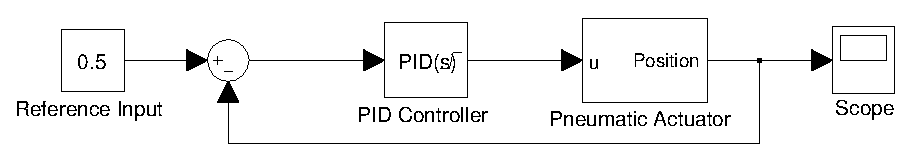
\includegraphics[scale=1]{implementation/figures/pneumatic_modelling1.eps}
\caption{Simulink model of the electro-pneumatic system.}
\label{fig:pneumatics_top_level}
\end{figure}

The three major components of the electro-pneumatic system are the \emph{PWM generator}, the \emph{solenoid valves}, and the \emph{pneumatic actuator}. Models of these systems are described further in the following sections.

\subsubsection{PWM Generator Model}

The PWM generator is used to provide the electrical control signals required by the solenoid valves to open and close. Our model of the PWM generator uses the instantaneous model presented by \citet{valve_models}. This model compares a generated saw-tooth signal $V_{saw}$ with the input signal $V_{in}$ over a time period $T_{saw}$ to obtain the pulse-width-modulated signal $U(t)$. The relationship is illustrated in Eq. \ref{eq:pwm_generation}.

\begin{equation}
\label{eq:pwm_generation}
U\left(t\right) = 
\begin{cases}
1 & V_{in}\left(t\right) \geq V_{saw}\left(t\right) \\
0 & V_{in}\left(t\right) < \left(t\right)
\end{cases}
\end{equation}

The Simulink model which implements Eq. \ref{eq:pwm_generation} can be seen in Fig. \ref{fig:pneumatics_pwm}. The input to the subsystem, shown as \emph{In1}, is $V_{in}$, and the output, shown as \emph{Out1} is the pulse width modulated signal $U(t)$. 

\begin{figure}[H]
\centering
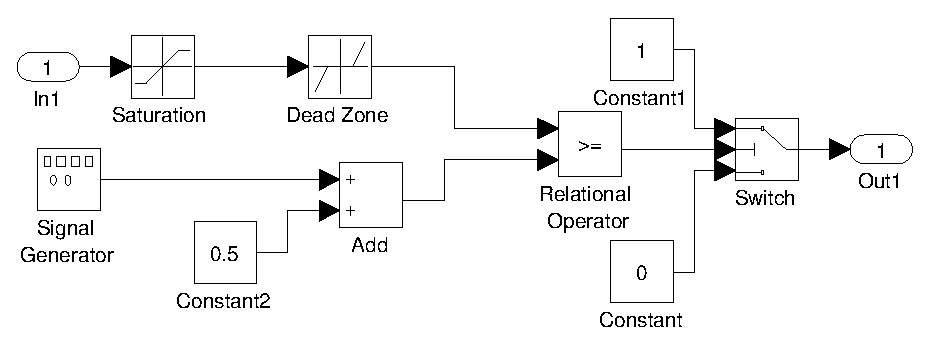
\includegraphics[scale=0.65]{implementation/figures/pneumatic_modelling2.eps}
\caption{Simulink model of the PWM generator.}
\label{fig:pneumatics_pwm}
\end{figure}

A saturation block limits the input signal $V_{in}$ to the range of \unit{[0..1]}{\volt}. A dead-zone block is present to account for the dead-zone present in the solenoid valve response to a PWM signal. If the pulse width is too short, the current through the solenoid cannot generate enough force to open the poppet, so the valve stays shut. This is a parameter of the solenoid valve, and was quantified experimentally by \cite{valve_models} as the minimum input signal $V_{in}$ required to open the valve. \Citet{accurate_position} also account for a minimum possible duty cycle in the solenoid valve input signal, known as $d_{min}$. This value can be calculated as:

\begin{equation}
  \label{eq:pwm_duty_min}
  d_{min}=\left(T_{vr}/T_{PWM}\right)\cdot100\%
\end{equation}

In this case, $T_{vr}$ is the time required by a solenoid valve to respond to an input, and $T_{PWM}$ the period of the PWM signal.

\nomenclature{$d_{min}$}{The minimum possible duty cycle of a solenoid's drive signal that will cause the valve to open.}
\nomenclature{$T_{vr}$}{The time required by a solenoid valve to respond to an input.}

The signal generator block in Fig. \ref{fig:pneumatics_pwm} outputs a triangle wave with peak-to-peak amplitude of \unit{1}{\volt}, which is then offset by \unit{0.5}{\volt}. The relational operator block then compares this with the input signal, and outputs the resulting PWM signal.

\subsubsection{Solenoid Valve Model}

An initial Simulink model of a solenoid valve was constructed based on the modelling equations described by \citet{valve_models} and the standard orifice equations for laminar and choked flow described in \cite{fluid_power}. However, it was too difficult to identify the system parameters cited in \cite{fluid_power} for our specific solenoid valves. The solenoid's data-sheet was not detailed enough, and the straight-forward approach to system identification used by \cite{valve_models} required specialized measuring equipment (such as an instantaneous mass flow meter) that we did not have access to.

The custom Simulink solenoid valve block was replaced with an approximate Simulink ``Simscape'' pneumatic valve block. This block could be configured with data obtained from the valve's data-sheets. 

\subsubsection{Pneumatic Actuator Model}

Simulink's pneumatic actuator subsystem is illustrated in Fig. \ref{fig:pneumatics_actuator}. Pre-built Simulink blocks from the Simscape package were used to model the dynamics of the actuator. \emph{Physical Port 1} (denoted by the octagonal port symbol with a ``1'' inside) in \ref{fig:pneumatics_actuator} represents the air inlet. \emph{Physical Ports 2 and 3} (denoted by the octagonal port symbols with a ``2'' and ``3'' inside, respectively) represent the displacement ports of the cylinder. \emph{Regular Port 1} (denoted by the rounded port symbol with a ``1'' inside) is used to display the displacement on a scope.

\begin{figure}[H]
\centering
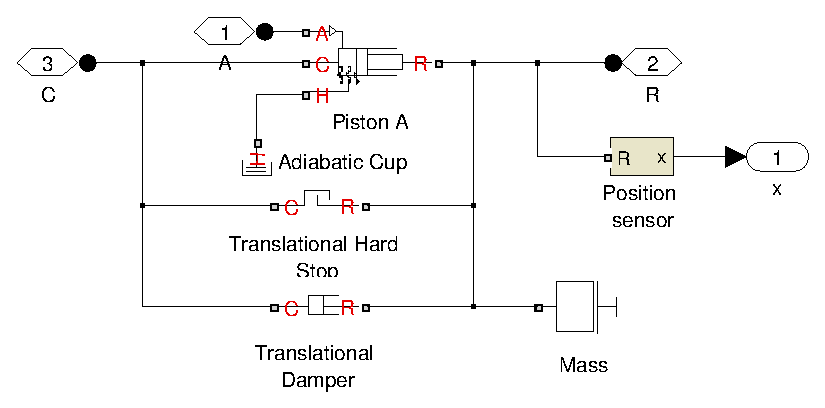
\includegraphics[scale=0.65]{implementation/figures/pneumatic_modelling3}
\caption{Simulink model of the pneumatic actuator.}
\label{fig:pneumatics_actuator}
\end{figure}

\subsubsection{Integrated Simulink Model}

The complete open-loop actuator model can be seen in Fig. \ref{fig:pneumatics_model_full}. The absolute value of the real-valued input $u$ is first fed to the PWM block. This signal is then converted into separate signals for each of the two solenoid valves in a way similar to the first PWM pulsing scheme presented by \citet{accurate_position}. The input to the subsystem $u$ is expected to range from -1 to 1. When $u\geq0$, the input to valve A is the pulse width modulated signal $U$, and the input to valve B is 0. When $u<0$, the opposite situation occurs.

\begin{figure}[H]
\centering
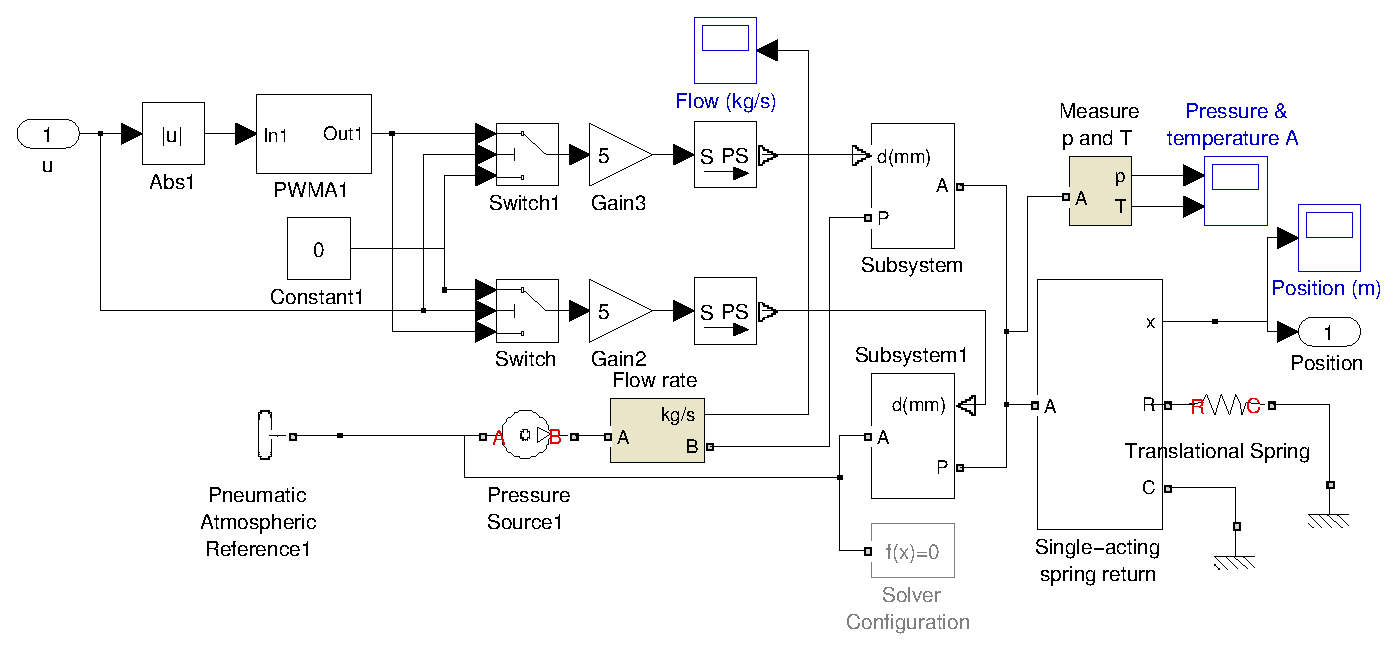
\includegraphics[scale=0.65]{implementation/figures/pneumatic_modelling4}
\caption{Simulink model of the full electro-pneumatic system.}
\label{fig:pneumatics_model_full}
\end{figure}

\subsection{Component Selection}

Selection of components was limited by budgetary constraints, however adequate solenoid valves and pneumatic actuators were found. These are detailed in the following sections.

\subsubsection{Solenoid Valves}

Solenoid valves and cylinders from SMC corp were chosen for the physical implementation of the design, specifically the \emph{VQZ115} series valve. Table \ref{tab:solenoid_specs} shows the specifications for this solenoid valve. A maximum operating frequency of \unit{20}{\hertz} was the fastest available solenoid that met the output force requirements while still being within the Formula SAE budget.

\begin{table}[H]
  \caption{Specifications of the SMC VQZ115 solenoid valve.\label{tab:solenoid_specs}}
  \centering

  \begin{tabular}{|l|l|}
  \hline
  Part & VQZ115-6L1-N1-PR \tabularnewline
  \hline
  Coil Voltage & \unit{12}{\volt} \tabularnewline
  \hline
  Configuration & 3-port Normally Closed \tabularnewline
  \hline
  Flow Coefficient & $C_v=\unit{0.23}{}$ \tabularnewline
  \hline
  Maximum Operating Frequency & \unit{20}{\hertz} \tabularnewline
  \hline
  Maximum Pressure & \unit{0.7}{\mega\pascal} \tabularnewline
  \hline
  \end{tabular}
\end{table}

\subsubsection{Pneumatic Actuators}

The pneumatic actuators specified for implementation are the same as used in the previous design, and are only briefly mentioned in this report. Specifications can be found in Table \ref{tab:cylinder_specs}. The clutch cylinder is specified with an internal magnet on the piston that interfaces magnetically with a membrane potentiometer, discussed next.

\begin{table}[H]
 \caption{Specifications of the pneumatic actuators used.\label{tab:cylinder_specs}}
  \centering
  \begin{tabular}{|l|l|l|l|}
   \hline
   Part & Bore Size & Stroke & Part Number \tabularnewline
    \hline
    \hline
    Shift actuator & 9/16`` & 2'' & NCMC056-0200 \tabularnewline
    \hline
    Clutch actuator & 3/4`` & 2'' & NCDMC075-0200 \tabularnewline
    \hline
  \end{tabular}
\end{table}

\subsubsection{Positional Feedback Sensors}

A ``MagnetoPot'' contact-less potentiometer from Spectra Symbal provides positional feedback from the clutch cylinder. The internal magnet in the cylinder interacts with the ``MagnetoPot'', which has a three-wire electrical interface similar to a standard potentiometer.


\section{Hardware Implementation\label{sec:Hardware-Implementation}}


\subsection{Methodology}

Commonality between modules, same life-support system.


\subsection{CAD Design}

Schematic capture and PCB layout using EagleCAD.


\subsection{Commonalities}

All 4 modules are implemented on custom printed circuit boards (PCBs) with an \emph{AT90CAN128} micro-controller from Atmel. Programming and debugging software on the microcontroller was done through a standard IEEE 1149.1 JTAG interface. The module is linked to the other system modules with a CAN bus. All inter-module communication is done over the CAN bus.

\subsubsection{Microcontroller}


\subsubsection{CAN Transceiver}


\subsubsection{Linear Regulator}


\subsubsection{Supervisor}


\subsubsection{Wiring Harness}


\subsection{Engine and Transmission Module}

<Picture of board>

Overview of physical implementation.


\subsubsection{High Current Solenoid Driver}


\subsubsection{Input Buffers}


\subsubsection{Traction Control Analogue Output}

The ECU allows a 0-5v analogue input to modify the allowable traction slip ratio from 0-100\% for the traction control.

The Engine module uses a simple SPI interfaced DAC from Texas Instruments, the TLV5623, to output the 0-5v analogue signal to the ECU.

The output voltage from the DAC is given by

\begin{equation}
V_{out}=2\cdot{V_{ref}}\,\frac{Code}{2^{n}}\,[V]
\end{equation}

where $V_{ref}$ is the reference voltage input to the chip, $n=8\,(bits)$, and $Code$ is the digital input value ranging from $0$ to $2^{n-1}$. Since we want to output $5\,[V]$ at fullscale input, \begin{equation} 2\cdot{V_{ref}}\,\frac{2^{7}}{2^{8}}=V_{ref}=5\,[V]\end{equation}.

The DC input resistance $R_{in}$ on the traction cut input pin on the ECU was measured using a series resistor with the input terminal to be $R_{in}\approx155k\Omega$. The output current of the DAC therefore will be at most $I_{out}=\frac{5v}{155k}\approx32.26\mu A$.

\subsection{Braking Module}

\begin{figure}[h]
\centering
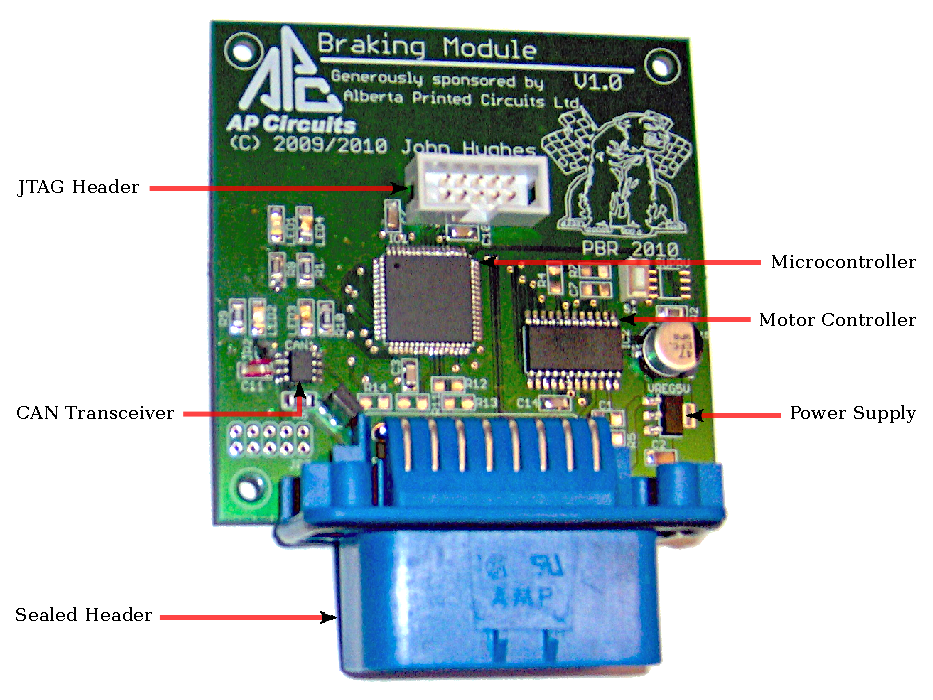
\includegraphics[scale=1]{implementation/figures/braking_pcb}
\caption{Populated Braking module PCB.}
\label{fig:braking_pcb}
\end{figure}

The braking module implementation was the simplest of the 4 modules in terms of electrical design. Only one special component on the board was required, a stepper motor controller/driver, and the interface to the microcontroller only required a handful of i/o lines. Additionally, a pressure transducer was also specified to facilitate measuring the hydraulic pressure in the brake lines. The components chosen for the braking module are listed in Table \ref{table:braking_module_components}.

Figure \ref{fig:braking_pcb} shows a photograph of the completed braking module circuit board, with all components soldered on. The simplicity of the electrical design is reflected in the fact that no additional corrections (other than for the CAN transceiver) were required for the module to be 100\% operational.

\begin{table}
  \caption{Braking module components.\label{table:braking_module_components}}
  \centering
  \begin{tabular}{|c|c|c|}
    \hline 
    Part & Manufacturer & Part Number\tabularnewline 
    \hline \hline
    Stepper Motor Controller/Driver & Allegro Microsystems & A3967 \tabularnewline
    \hline
  \end{tabular}
\end{table}

\subsubsection{Stepper Motor Driver}

In order to meet the design goal of having the implementation be flexible in terms of which stepper motor would be used in the system, a current-sensing stepper motor controller/driver component was used in the circuit design. The current sense capability allows us to fix the input voltage in the circuit design, and afterwards adjust the current drive by changing resistor values in the current-sense feedback loop. 

The A3967 "Microstepping Driver with Translator" was chosen to drive the stepper motor for several reasons. The A3967 integrates a microstepping controller with dual H-Bridge output stages into one package. This simplified the potential circuit design. The H-Bridge output transistors can supply up to $\pm\unit{750}{\milli\ampere}$ of current at up to \unit{30}{\volt} \cite{A3967}. This flexibility was desirable.

\paragraph{Current Control}
\nomenclature{$R_{sense}$}{Value of the current sense resistors in the Braking Module's stepper motor circuit.}
\nomenclature{$I_{TRIP}max$}{Maximum current allowed to flow into the Braking Module's stepper motor before the PWM circuit shuts the output stage off.}

The current control feature of the A3967 works by sensing the current through a sense resistor, $R_{sense}$, and varies the duty cycle of a fixed off-time PWM circuit, which controls the output from the H-Bridge stages.

The value of the sense resistor was determined by an equation recommended in the datasheet:
\begin{equation}
R_{sense}=\frac{0.5}{I_{TRIP}max}
\end{equation}
where $I_{TRIP}max$ is the maximum current allowed to flow into the motor before the PWM circuit shuts the output stage off.

\subsubsection{Analogue-to-Digital Converter}


\subsubsection{End-of-Travel Microswitches}

\subsection{Telemetry Module}


\subsubsection{Wireless Modem}

To meet the range and data throughput requirements for the telemetry system, an XBee Pro wireles modem was used. The XBee requires 3.3v I/O levels and power supply, and so a second linear voltage regulator was used in the design, the LT1521 from Linear Technology. Since the AT90CAN129 has only 2 built-in UARTS that were used for the RS232 interfaces to the ECU and DAQ, an third external UART was added to the design. The MAX3100 is a SPI-interfaced UART with an 8 word deep FIFO buffer. It is interfaced to the AT90CAN128's SPI pins and has an active-low IRQ line connected to external interrupt line EXT7 on the microcontroller. 

The wireless transmitter is an XBee Pro Modem from Digi International. The modem is in a package designed for mounting on a printed circuit board, and is attached to the telemetry module directly. This modems requires a 3.3V power supply. and consumes at most 215mA of current during transmit. Since the common module hardware only provides power for 5V devices, the telemetry module has a second LDO regulator providing 3.3V. A separate antenna port is connected to the modem and mounted in the side of the module enclosure.



\subsubsection{External SPI USART}


\subsubsection{Two-Channel ECU and DAC USART}

\subsection{Driver Interface Module}


\subsubsection{Steering Wheel Unit}


\subsubsection{LCD Module Bias Circuit}

The LCD screen requires a large bias voltage of +22V.

A Linear Technology LT1615 step-up DC/DC converter was chosen as the centre of a boost converter circuit for the LCD.


\paragraph{Inductor Selection}

\begin{equation}
L=\frac{V_{out}-V_{in(min)}+V_{D}}{I_{limit}}\cdot t_{off}\label{IndSel}
\end{equation}


Using (\ref{IndSel}) with $V_{D}=0.4V$, $I_{limit}=350mA$, $t_{off}=400ns$, $V_{out}=+22V$, and $V_{in(min)}=11.5V$ gives $L\approx12.45\mu{H}$. The datasheet however suggests a value slightly smaller than calculated should be suitable with only slight decrease in maximum output current. Since the LCD requires very little current, we used an inductor value of $10\mu H$.


\paragraph{Output Voltage}

To obtain a $V_{bias}$ of $+22V$, two resistors in the bias circuit provide a voltage divided feedback path from the output to the FB pin on the LT1615. The eqation relating the output voltage with the resistor values is

\begin{equation}
R_{1}=R_{2}\cdot\left(\frac{V_{bias}}{1.23}-1\right)
\end{equation}

 $R_{1}$ was chosen to be $2M\Omega$ to limit current flowing from the output to ground, and a suitable $R_{1}$ of $118k\Omega$ was found.


\subsubsection{LCD Module Data Interface}

The LCD's 8-bit interface was suitable to be connected to the AT90's external memory interface. This way the LCD becomes a memory-mapped periferal to the AT90, and all the control signals (Read and Write strobes, etc.), are handled by the memory controller.

The AT90's external memory interface uses Port A pins 0-7 as a multiplexed data and address bus which must be demultiplexed in order to offer seperate address and data busses. In operation, the external memory interface first puts out the address on the combined bus, followed by the data. The ALE (Address Latch Enable) signal signifies the difference \cite{AT90CAN}.

In order to provide seperate address and data busses for the LCD controller, a fast octal D-Type latch from NXP was chosen to latch the address from the AT90. The width of the ALE pulse, $t_{LHLL}$, provided by the AT90, is specified in the datasheet as

\begin{equation}
t_{LHLL}=t_{CLCL}-15\, ns
\end{equation}

 where $t_{CLCL}$ is the clock period. With the clock running at $16\, MHz$, $t_{LHLL}=48\, ns$.

The 74LVC373A latch from NXP requires a minimum LE pulse width of $4.5\, ns$, so is suitable as a demultiplexing interface.

The external memory on the AT90CAN128 starts at address 0x1100h, and there are two possible registers to read/write to on the LCD controller. The LCD controller therefore has it's single address select pin connected to the LSB of the address lines output from the latch. Since only two addresses are required, the upper 8 address lines of the external memory interface were not used.

A logical combination of the lower byte address lines will be connected to the CS (Chip Select) line on the LCD controller. Since the external memory controller only outputs control signals when the requested memory operation is in external space, it is safe to ignore the upper byte address lines.

It was chosen to tie the 2nd bit of the address lines to CS, which provides the following table of operations when interacting with the LCD controller:

\begin{table}
\begin{centering}
\caption{Memory-mapped LCD Interface}

\par\end{centering}

\centering{}\begin{tabular}{|l|l|l|}
\hline 
Address  & Read Function  & Write Function\tabularnewline
\hline
\hline 
0x1102  & Status flag read  & Display data and parameter write\tabularnewline
\hline 
0x1103  & Display dada and cursor address read  & Command write\tabularnewline
\hline
\end{tabular}
\end{table}

\subsubsection{Input Knobs and Buttons}


\subsubsection{Paddle Shifters}

\section{Software Implementation\label{sec:Software-Implementation}}


\subsection{Methodology}


\subsection{Toolchain}


\subsection{Common Low-Level Drivers}


\subsubsection{CAN Driver}


\subsubsection{EEPROM Driver}


\subsubsection{SPI Driver}


\subsection{Engine and Transmission Module}

<Software interface map>


\subsubsection{Transmission Manager}


\subsubsection{Intake Manager}


\subsubsection{Starter Manager}


\subsubsection{Event Scheduler}


\subsubsection{CAN Interface}

<Data flow diagram>


\subsubsection{PWM Generator}

An efficient method was devised to generate 2 synchronized PWM signals from the L9822E driver chip. The $32\, kHz$ external crystal was used as the input to the 8-bit TIM2 timer periferal on the microcontroller. The input to the timer was first scaled by 8 which provided a timebase:
\begin{equation}
TB=\frac{32.768\, kHz}{8}=4.096\, kHz
\end{equation}

The timebase period is then given by:
\begin{equation}
\frac{1}{TB}\approx244\,\mu{S}
\end{equation}

We then define a constant scaling factor for the PWM generator:
\begin{equation}
{PWM\_DUTY\_SCALE}=\frac{T_{PWM}}{TB}\approx205
\end{equation}

By loading the timers compare register with with a value scaled with the constant scaling factor, we can cause the timer to generate an interrupt precisely when a level change in the PWM is required.

When generating 2 waveforms with the same timer periferal, 8 combinations of duty cycles of channels A and B were identified, and can be seen in Figure \ref{fig:pwm_cases}.

Since the waveforms are synchronized, it can be seen that there are only 2 cases where 3 transitions per period are required, corresponding to \ref{fig:pwm_cases_1} and \ref{fig:pwm_cases_2}. This happens when both channels have $0<Duty<100\%$. 2 cases are also apparent when no transitions are required, shown in \ref{fig:pwm_cases_7} and \ref{fig:pwm_cases_8}.

An efficient generating routine was constructed to effect the level transitions and to reset the timer to interrupt at the next transition. For the two cases requiring 3 transitions per period, the timer interrupts 3 times per period. For the two cases where both channels have duty cycle between 0 and 100\%, the routine still interrupts once to allow for a change in duty cycle. For the rest of the cases described, the timer only interrupts twice per PWM period.

\input{implementation/figures/pwm_cases.tex}

\subsubsection{Main Control Loop}


\subsection{Braking Module}


\subsubsection{Bias Library}


\paragraph{Bias Position Request}

<Position request flow chart>


\paragraph{Bias Calibration}

<Calibration flow chart>


\subsubsection{Pressure Library}


\paragraph{Periodic Pressure Output}


\paragraph{Pressure Calibration}

<Calibration flow chart>


\subsubsection{CAN Interface}

<Data flow diagram>


\subsubsection{Main Control Loop}


\subsection{Telemetry Module}

The primary objective of the software running on the Telemetry Module is to push data around from various sources to various sinks. It uses the interrupt-driven USART drivers written for the on-board USARTs of the AT90CAN128, as well as the MAX3100 external USART extensively. These USART drivers are discussed in section ?? 

\begin{figure}[H]
\centering
\input{implementation/figures/telemetry_software_block.tex}
\caption{Telemetry software overview.}
\label{fig:telemetry_software_implementation}
\end{figure}

\subsubsection{Internal USART Driver}

\begin{figure}[]
\centering
\input{implementation/figures/usart_driver_flow.tex}
\caption{Basic USART interrupt flow diagram.}
\label{fig:usart_driver_flow}
\end{figure}


\subsubsection{MAX3100 Driver}

An interrupt-driven driver was written to interface with the MAX3100 uart chip which allows asynchronous serial communication with the XBee modem on the Telemetry Module. The same circular buffer approach as with the internal USART drivers was taken, and in fact the drivers use very similar buffering code. Additionally, the software interfaces to the drivers were made as close as possible to allow interchangability by the main module software.

The datahseet for the MAX3100 states that the minimum SPI Clock period is $t_{CP}=238\, ns$, which results in a maximum frequency of approximately $4.2\, MHz$ \cite{MAX3100}. The SPI periferal was thus set to use 1/4 of the system clocks frequency resulting in $4\, MHz$.

The MAX3100 was configured to operate at 115,200 kBaud, which was matched with the XBee modem's interface rate. A simple throughput stress test was performed that continuously wrote data in 16 byte chunks into the driver's software transmit buffer. A fixed-length 32 byte buffer was never overrun with this test, and an actual data throughput of $8.251\, kB/s$ was observed with a logic analyser.

\subsubsection{Xbee Library}

In order to facilitate routing data to and from multiple sources and sinks, it was determined that the Xbee would need to be interfaced using the special "API" mode described in the Xbee documentation \cite{XBeeManual}. The API mode is characterized by a packet interface that needed to be implemented in software. A library was written to implement two critical pieces of functionality:

\begin{enumerate}
\item to set the modem into API mode operation and manage the modem's operating state;
\item and to send and receive packetized data from the modem on behalf of the user software as per the Xbee's API specification \cite{XBeeManual};
\end{enumerate}

The Xbee library implements the binary packet protocol described in the XBee manual, and is able to send and receive unicast and multicast packets. The driver is only capable of sending packets to 16-bit addresses. Full 64-bit address mode was not implemented as the address space was not required in our 3 node network. The driver is also capable of sending command-type packets to the modem and reading the response.

Managing the modem's state was implemented as a state machine. Since minimal functionality was required, only a handful of modem commands were implemented. The driver is able to push the modem into API mode, after which all communication is done using the packet interface.

The modem commands implemented are listed in Table \ref{tab:xbee_commands}.

\begin{table}
\caption{Implemented Xbee modem commands.\label{tab:xbee_commands}}
\centering{}
\begin{tabular}{|l|l|}
\hline 
Command & Description \tabularnewline
\hline
\hline
AP & Set and read the API mode state \tabularnewline
\hline
CH & Set and read the RF channel \tabularnewline
\hline 
ID & Set and read the PAN (Personal Area Network) ID \tabularnewline
\hline
MY & Set and read the modems local address \tabularnewline
\hline
\end{tabular}
\end{table}

Similar to the rest of the software drivers implemented, the Xbee library uses callbacks to provide the user software with incoming data. Function pointers are used to connect the library to a UART, which makes it possible to reconfigure the library to use a different USART on-the-fly.

\subsubsection{DAC Library}

To reduce the implementation work required by us, we asked David Schilling, a computer science student on the Formula SAE team, to write the DAC software library to read and write the DAC's serial format, given the requirements described in Section \ref{sec:Telemetry-Module-Design}.

The DAC library maintains it's own buffer of incoming DAC data. We also asked Dave to provide seperate functions for buffering incoming data, and for processing that data. This seperation allowed the library to be easily tied in with the rest of the system software on the telemetry module: adding a data to the DAC buffer occurs whenever the internal USART driver interrupts with a new byte, and processing is called from the mainline loop.

\subsubsection{Main Control Loop}


\subsection{Driver Interface Module}


\subsubsection{LCD Module Library}


\subsubsection{Graphics and Fonts Library}


\subsubsection{I/O Library}


\subsubsection{Vehicle Diagnostics Library}


\subsubsection{Vehicle Parameter Library}


\subsubsection{Vehicle Dynamic Mode}


\subsubsection{CAN Interface}


\subsubsection{Main Control Loop}

\section{CAN Diagnostic Tool}
\label{sec:implementation_candt}

\subsection{Overview}

\subsection{Scheduling}

\subsection{Injecting}

\subsection{Snooping}


\chapter{Results and Discussion}


\section{Transmission}


\subsection{Shift Speed}


\subsection{Launch Control}


\subsection{Neutral Find}


\subsection{Anti-Stall}


\subsection{Electropneumatics}


\section{Intake}


\section{Starter}


\section{Braking}


\subsection{Bias Adjustment}


\subsection{Calibration}


\section{Telemetry}


\subsection{Data Interfaces}


\subsubsection{ECU }


\subsubsection{DAC }


\subsubsection{Wireless Data Link}


\section{Driver Interface}


\subsection{Driver Controls}


\subsection{Vehicle Dynamic Adjustment}


\subsection{Diagnostic Information}


\subsection{LCD Interface}

\subsubsection{Bench Experiments}

To verify the LCD data interface circuitry before the final Driver Interface module hardware had been completed, a bench test of the LCD module with an ARM7 development board was conducted. The bus interface as designed in Sec.\ \ref{sec:lcd_module_data_interface} was implemented on a breadboard: a latch and level shifter were used as in the Driver Interface module circuit design, and an FPC cable adapter was constructed with the aide of the tech shop to allow connecting the LCD module to the breadboard. The GPIO pins on the ARM7 development board (shown in red in Fig.\ \ref{fig:can_bench_test}) were used to bit-bang the data interface to the LCD. This test setup was used to write the initial LCD module code used in the final Driver Interface module implementation.

\begin{figure}[h!]
\centering
\subfigure[LCD Bench test]{
  \label{fig:lcd_bench_test}
  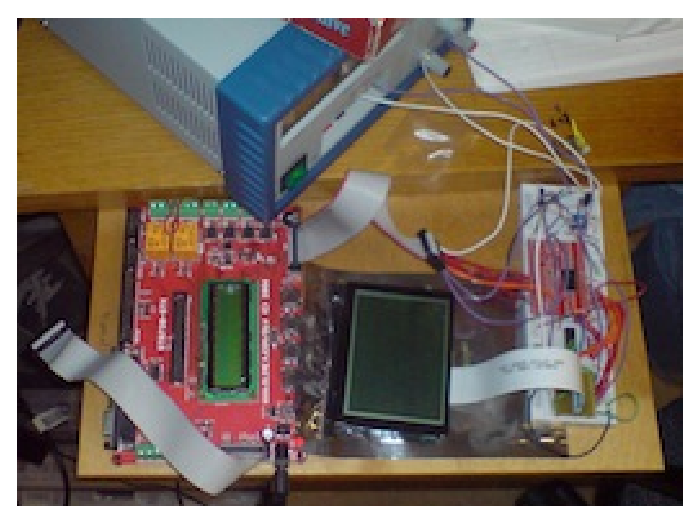
\includegraphics[width=2.5in,keepaspectratio]{experimental_results/figures/lcd_bench_test.eps}
}
\subfigure[CAN Bench test]{
  \label{fig:can_bench_test}
  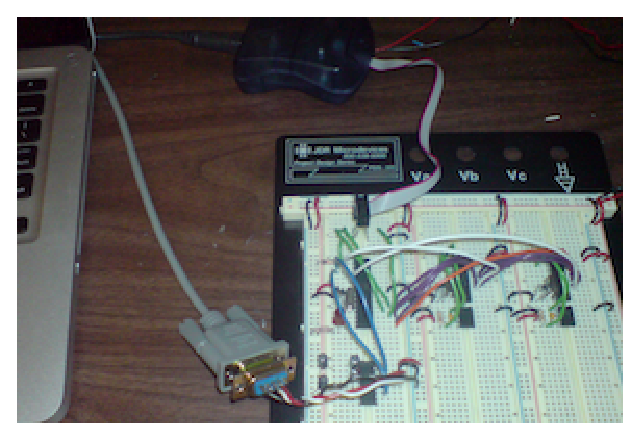
\includegraphics[width=2.5in,keepaspectratio]{experimental_results/figures/can_bench_test.eps}
}
\caption{Bench experiments conducted during the implementation phase.}
\label{fig:bench_experiments}
\end{figure}

Once all the hardware bugs with the Driver Interface module had been corrected, it was possible to continue writing the LCD interfacing software that had been started during the initial LCD testing. The external memory interface circuitry described in Sec.\ \label{sec:lcd_module_data_interface} worked without issue. Figure \ref{fig:driver_interface_lcd} shows the LCD displaying a sample bitmap from the manufacturer.

\begin{figure}[h]
 \centering
 \includegraphics[width=6in,keepaspectratio]{experimental_results/figures/driver_interface_lcd.eps}
 \caption{Testing the LCD on the Driver Interface module.}
 \label{fig:driver_interface_lcd}
\end{figure}

\section{Implementation Issues Encountered}


\subsection{Hardware Implementation Issues}


\subsubsection{CAN Transciever Schematic Error}


\subsubsection{Driver Interface LCD Reset Line}


\subsubsection{Telemetry RS-232 Transciever Schematic Error}


\subsection{Interrupt Starvation on the Telemetry Module}

Although initial average data throughput rates for both the DAC and the ECU were measured as part of the research done at the beginning of the project, non-trivial buffering issues did arise in the implementation of the telemetry module software. After several weeks of work spent debugging throughput problems with the module software, and with the aide of a protocol analyser, the root of the problem was tracked down. The AT90CAN microcontroller's interrupt vectors are fixed at the factory, therefore the priority of interrupts on the microcontroller is fixed. Unfortunately this lead to a resource starvation issue. The MAX3100 UART uses an external interrupt line, which has priority over the internal UART interrupts. When there is data in the MAX3100's transmit buffer, it will starve the internal UART interrupt to a certain extent. This was investigated by saturating the MAX3100 output buffer with a constant stream of data, and then inputting some bytes to the internal UART. Single input bytes were read properly, but any long stream of incoming bytes (more than 4 in a row) would cause hardware input buffer overruns in the built-in UART, and incoming data would be lost.

\begin{figure}[ht]
  \centering
  \label{fig:ecu_data}
  \begin{tikztimingtable} %[timing/nice tabs]
    $ECU_{Rx}$ & Z 10D{Polling sequence (7 bytes)} 14F Z \\
    $ECU_{Tx}$ & 12Z 6D{Reply sequence} ;[dotted] 2D{...}; 5D{(539 bytes)} Z\\
    \extracode
      %\tableheader{Signal}{Timing}
      \tablerules
  \end{tikztimingtable}
  \caption{ECU Serial Data Example}
\end{figure}

Based on this knowledge, we were able to classify conditions where the software would be unable to accurately process the incoming data. Unfortunately the method that the ECU transmits it's data falls within this characterization. When the ECU is communicating with the DTASWin software, the software will send a handful of bytes (around 7) to the ECU, and the ECU will reply with one large packet of approximately 540 bytes. If the MAX3100 is transmitting a large amount of data when this large packet comes in, bytes will be lost from the interrupt starvation issue.

Having determined the problem, several options lay before us to resolve the issue:
\begin{itemize}
  \item By lumping the ISR handlers for both the internal UART and the MAX3100 together, it would be possible to conditionally alter the priority of the processing to allow the incoming data to take precedence. This would however override the natural encapsulation that the two drivers had, and would require writing specialized drivers for use only on the telemetry module.
  \item Throttling the transmission of data to the MAX3100 by sequenced enabling and disabling of the interrupt could also reduce the starvation issue, but getting the sequencing and timing right would be difficult and more than likely result in further problems.
\end{itemize}


\subsection{CAN Driver Problems}

\chapter{Conclusion}

\chapter{Future Work}

%%% References

\clearpage
\bibliographystyle{IEEEtranN}
%\bibliographystyle{ieeetr}
%\bibliographystyle{plainnat}
%\renewcommand{\referencename}{References}
\renewcommand{\bibname}{References}
\addcontentsline{toc}{chapter}{\bibname}
\bibliography{reference/datasheets,reference/literature,IEEEfull}

%%% Appendix

\appendix

\chapter{Description of Attached Materials}

Attached DVD, etc.


\chapter{CAN Protocol Specification}

\chapter{S-Series CAN Stream Specification}

\chapter{Analysis of Clutch Operation\label{cha:clutch_analysis}}

Equations of motion governing the clutch dynamics are:

\begin{equation}\label{eq:clutch_dynamics_a}
  J_c\dot{\omega}_c=T_c-T_d-b_c\cdot\left(\omega_c-\omega_t\right)
\end{equation}

\begin{equation}\label{eq:clutch_dynamics_b}
  \dot{T}_d=k\left(\phi_d\right)\cdot\left(\omega_c-\omega_t\right),
\end{equation}

where $J_c$ is the inertia of the clutch plates, $T_c$ the torque transmitted through the clutch, $b_c$ the clutch damping rate, and $\omega_c$ and $\omega_t$ are speeds of the clutch plates and transmission respectively \cite{clutch_control}.

A major point of interest in the operation of the clutch is the transition from fully disengaged to fully engaged, and vice-versa. In this state the clutch plates slip against each other as one rotates faster. \Citet{clutch_control} describe the torque transmitted through the clutch in slipping, $T_c{slip}$, as

\begin{equation}\label{eq:clutch_slip}
  T_c{slip}=F_n\mu R_a \cdot sgn\left(\omega_e-\omega_c\right),
\end{equation}

where $F_n$ is the normal force on the clutch plates, $\mu$ the coefficient of friction on the plate surfaces, and $R_a$ the radius of the plates, and $\omega_e$ and $\omega_c$ are the rotational velocities of the engine, and clutch discs, respectively. This shows that the amount of torque transmitted depends dynamically on the normal force $F_n$, which is proportional to the spring force pushing the plates together.

The second state of interested, as described by \cite{clutch_control}, is when the clutch is fully engaged and the plates are locked rotating at the same speed. The equation of motion for the engine, where the engine inertia $J_e$ is driven by the engine torque $T_e$ is given by:

\begin{equation}\label{eq:engine_motion}
  J_e\dot{\omega}_e=T_e-T_c.
\end{equation}

In the fully engaged state, $\omega_e=\omega_c=\omega$, a degree of freedom is removed, and by combining \eqref{eq:clutch_dynamics_a} and \eqref{eq:engine_motion} we obtain:

\begin{equation}
  \left(J_e+J_c\right)\dot{\omega}=T_e-Td-b_c\cdot\left(\omega\right),
\end{equation}

which shows that the system torque acts on the combined inertia of the plates as a single unit as the engine and transmission rotate at the same speed.

\phantomsection \label{cha:attached_dvd}
\addcontentsline{toc}{chapter}{Attached DVD}

% Finito

\end{document}